%%%%%%%%%%%%%%%%%%%%%%%%%%%%%%%%%%%%%%%%%%%%%%%%%%%%%%%%%%%%%%%%%%%%%%%%
\chapter{Approximation of the Diagonal of a Laplacian’s Pseudoinverse for Complex Network Analysis}
\label{ch:electrical-closeness}
% Labels: approximate, static, algebraic, parallel
%%%%%%%%%%%%%%%%%%%%%%%%%%%%%%%%%%%%%%%%%%%%%%%%%%%%%%%%%%%%%%%%%%%%%%%%

\section{Introduction}
\label{sec:el-clos:intro}
%
In this chapter, we address the problem of approximating electrical centrality
measures for the analysis of complex networks -- also known as
small-world networks, \ie graphs whose diameter is bounded by $\Oh(\log n)$,
see \Cref{sec:intro:methodology}.
The small-world feature is typical of many real-world
networks such as social networks, biological networks, information networks,
\etc~\cite{newman2018networks}. As described in \Cref{sec:centrality-measures},
many centrality measures exist, some of which are based on shortest paths (or
shortest-path distances) while others consider paths of arbitrary lengths.
Electrical centrality measures interpret the graph as an electrical
network~\cite{lovasz1993random} and thus fall in the latter category. Here we
consider two electrical centrality measures: electrical closeness
centrality ($\elclos$)~\cite{DBLP:conf/stacs/BrandesF05} -- \aka current-flow
closeness or information centrality~\cite{stephenson1989rethinking} -- and
forest closeness centrality ($\fclosp$)~\cite{DBLP:conf/icdm/JinBZ19}.

\paragraph{Electrical Closeness}
The electrical closeness of a vertex $u \in V$ (see
\Cref{eq:electrical-closeness}) is defined as the reciprocal of the average
effective resistance $\rdist(u, \cdot)$ from $u$ to all other
vertices.\footnote{We remark that effective resistance
has numerous applications well beyond its usage in electrical centrality measures -- cf.
Refs.~\cite{DBLP:conf/innovations/AlevALG18,DBLP:journals/siamrev/GhoshBS08}.}
The effective resistance between two vertices $u, v\in V$ can be computed by solving
the linear system $\Lapl\vect{x} = \cunit{u} - \cunit{v}$ for $\vect{x}$, where
$\cunit{z}$ is the canonical unit vector for vertex $z$. Then,
$\rdist(u, v) = \vect{x}[u] - \vect{x}[v]$.
It is well-known that $\Lapl$ does not have full rank and is thus not invertible.
Its Moore-Penrose pseudoinverse~\cite{DBLP:books/daglib/0086372} $\Linv$,
however, can be used to compute $\rdist(u, v)$ as shown in
\Cref{eq:eff-res-laplinv}.

A straightforward way to compute the electrical closeness of any vertex would
be to compute $\Linv$ which, without exploiting the structure of $\Lapl$,
\change{takes} in practice \change{cubic time in $n$}, cf. Ref.
\cite{DBLP:conf/cocoa/RanjanZB14}. Further, this strategy would require
$\change{\Theta(n^2)}$ memory since $\Linv$ is in general a dense matrix --
even for sparse $\Lapl$. Therefore, full (pseudo)inversion is clearly limited
to small inputs.

Conceptually similar to inversion would be to solve $\Theta(n)$ Laplacian linear systems.
Fewer linear systems suffice in applications with lower accuracy requirements:
the Johnson-Lindenstrauss Transform (JLT) combined with a fast Laplacian solver (such as
Ref.~\cite{DBLP:conf/stoc/CohenKMPPRX14}) achieve
a relative approximation guarantee by solving $\Oh(\log n /\epsilon^2)$
systems~\cite{DBLP:journals/siamcomp/SpielmanS11} in $\tilde{\Oh}(m\log^{1/2}
n \log (1/\epsilon))$ time each, where $\tilde{\Oh}(\cdot)$ hides a
$\Oh((\log\log n)^{3 + \delta})$ factor for $\delta > 0$.

As pointed out by Bozzo and Franceschet~\cite{DBLP:journals/socnet/BozzoF13},
the (only) relevant part of $\Linv$ for computing the electrical closeness is
its diagonal -- we will see that this is true for other electrical centrality
measures as well. Numerical methods for sampling-based approximation of the
diagonal of implicitly given matrices already exist~\cite{bekas2007estimator}.
Yet, for our purpose, they solve $\Oh(\log n /\epsilon^2)$ linear system as
well to obtain an $\epsilon$-approximation with high probability.
%
While Laplacian linear systems can be solved independently in parallel, their solution can
still be time-consuming in practice, in part due to high constant overheads hidden
in the $\Oh$-notation.


\paragraph{Forest Closeness}
Forest closeness (see \Cref{eq:forest-closeness}) is based on the forest distance,
a metric introduced by Chebotarev and Shamis~\cite{chebotarev2000forest}.
It is defined as closeness centrality where the shortest-path distance is replaced
by the forest distance.
In sociology, forest distances are shown to effectively capture sensitive relationship indices
such as social proximity and group cohesion~\cite{DBLP:journals/corr/abs-math-0602070}.
Hence, forest closeness has two main advantages over many other centrality
measures~\cite{DBLP:conf/icdm/JinBZ19}: (i) unlike electrical closeness, it can
handle disconnected graphs out of the box and, by considering not only shortest
paths, (ii) it has a high discriminative power.

Jin \etal~\cite{DBLP:conf/icdm/JinBZ19} provided an approximation algorithm for
forest closeness centrality with nearly-linear time complexity. Similarly to
the aforementioned strategy for electrical closeness, their algorithm uses the
JLT and fast linear solvers; it is, however, still time-consuming. For example,
in their experimental study~\cite{DBLP:conf/icdm/JinBZ19}, graphs with
$\approx$ 1M to $\approx$ 2-3M edges require more than $\numprint{2.3}$ to
$\numprint{4.7}$ \emph{hours} for a reasonably accurate ranking. Clearly, this
hardly scales to larger graphs with \change{more than a few million edges}.

As already realized by Chebotarev and Shamis~\cite{chebotarev2000forest},
forest distance is closely connected to effective resistance. In particular, as
we describe in \Cref{sec:el-clos:forest-clos-extension}, any algorithm that
computes the electrical closeness can easily be adapted to compute the forest
closeness with just an additional linear-time overhead.

\subsection{Related Work}
\paragraph{Solving Laplacian Systems}
As mentioned above, a straightforward approach to compute electrical closeness
is to compute $\Linv$ by solving a number of Laplacian systems.
Brandes and Fleischer~\cite{DBLP:conf/stacs/BrandesF05} compute electrical closeness
from the solution of $n$ linear systems using Conjugate Gradient (CG) in $\Oh(mn\sqrt{\kappa})$,
where $\kappa$ is the condition number of the appropriately preconditioned Laplacian
matrix.\footnote{Brandes and Fleischer provide a rough estimate of $\kappa$
as $\Theta(n)$, leading to a total time of $\Oh(mn^{\numprint{1.5}})$.}
%
Later, Spielman and Srivastava~\cite{DBLP:journals/siamcomp/SpielmanS11}
proposed an approximation algorithm to compute effective resistance distances.
The main components of the algorithm are (i) a dimension reduction with
JLT~\cite{johnson1984extensions} and (ii) the use of a fast
Laplacian solver for $\Oh(\log n/\epsilon^2)$ Laplacian systems. The algorithm
approximates effective resistance values for all edges with a factor of $(1 \pm
\epsilon)$ in $\Oh(I(n, m)\log n/\epsilon^2)$ time, where $I(n, m)$ is the
running time of the Laplacian solver, assuming that the solution of the
Laplacian systems is exact. With an approximate Laplacian solution, the algorithm
yields a $(1 + \epsilon)^2$-approximation. Significant progress in the development
of Laplacian solvers with theoretical guarantees~\cite{DBLP:conf/stoc/CohenKMPPRX14,
DBLP:conf/stoc/KelnerOSZ13,DBLP:conf/focs/KoutisMP11,DBLP:journals/siamcomp/KoutisMP14,
DBLP:conf/stoc/KyngLPSS16}
has resulted in the currently best one running in $\Oh(m\log^{1/2}n \log
1/\epsilon)$ time (up to polylogarithmic
factors)~\cite{DBLP:conf/stoc/CohenKMPPRX14}.
%
Parallel algorithms for solving linear systems on the more general SDD matrices
also exist in the
literature~\cite{DBLP:conf/spaa/BlellochGKMPT11,DBLP:conf/stoc/PengS14}. To
date, the fastest algorithms for electrical closeness and spanning edge
centrality\footnote{The spanning edge centrality of an edge $e$ in a graph $G$
is defined as the number of spanning trees in $G$ that contain $e$ and it
is equivalent to the effective resistance of
$e$~\cite{DBLP:conf/www/MavroforakisGKT15}.}
extend the idea of Spielman and
Srivastava~\cite{DBLP:conf/siamcsc/BergaminiWLM16,
DBLP:conf/ijcai/HayashiAY16,DBLP:conf/www/MavroforakisGKT15}
-- similar ideas are also used for centrality measures based on the Kirchhoff
index, see \Cref{sec:el-clos:generalizations}. Since theoretical Laplacian
solvers rely on heavily graph-theoretic machinery such as low-stretch spanning
trees, multigrid
solvers~\cite{DBLP:conf/siamcsc/BergaminiWLM16,
DBLP:conf/isvc/KoutisMT09,DBLP:journals/siamsc/LivneB12}
are used in practice instead.

\paragraph{Diagonal Estimation}
Recall that only the diagonal of $\Linv$ [or of $\Fmat$, resp.] is enough to
compute the electrical closeness -- or, in case of the Kirchhoff index, only
the sum of $\diag{\Linv}$, \ie the trace $\tr{\Linv}$ is required -- [or the
forest closeness].
%
Algorithms that approximate the diagonal (or the trace) of matrices that are
only implicitly available often use iterative
methods~\cite{DBLP:journals/na/SidjeS11}, sparse direct
methods~\cite{DBLP:journals/siamsc/AmestoyDLR15,DBLP:journals/pc/Jacquelin0018},
Monte Carlo~\cite{hutchinson1989stochastic} or deterministic probing
techniques~\cite{bekas2007estimator,bekas2007estimator}.
%
A popular approach is the standard Monte-Carlo method for the trace of a matrix \mat{B}, due to
Hutchinson~\cite{hutchinson1989stochastic}. The idea is to estimate the trace of \mat{B} by
observing the action of \mat{B} (in terms of matrix-vector products) on a sufficiently large
sample of random vectors. In our case, this would require to solve a large number of Laplacian
linear systems with random vectors as right-hand sides. Avron and Toledo~\cite{DBLP:journals/jacm/AvronT11}
proved that the method requires $\Oh(\log n /\epsilon^2)$ samples to achieve a maximum error
of $\epsilon$ with probability at least $1 - \delta$. The approach from Hutchinson~\cite{hutchinson1989stochastic}
was extended by Bekas \etal~\cite{bekas2007estimator} for estimating \diag{\mat{B}}.
Finally, Barthelem\'e \etal~\cite{barthelme2019estimating} proposed a combinatorial algorithm to
approximate the trace (not the diagonal) of the inverse of a matrix closely related to the Laplacian.
Their algorithm can be seen as a special case of our algorithm in a situation where a universal
vertex exists (\ie a vertex connected to all the other vertices of the graph).

\subsection{Contribution and Outline}
We introduce a new algorithm for approximating \diag{\Linv} of a Laplacian matrix \Lapl
that corresponds to weighted undirected graphs (\Cref{sec:el-clos:apx-algo}). Our main technique
is the approximation of effective resistances between a pivot vertex $u\in V$ and
all other vertices of $G$.
It is based on sampling uniform (= random) spanning trees (USTs).
The resulting algorithm is highly parallel and (almost) purely combinatorial -- it relies on the
connection between Laplacian linear systems, effective resistances, and USTs.
Because effective resistance also plays a major role in \emph{normalized
random-walk betweenness}~\cite{DBLP:conf/complexnetworks/NarayanS18}
and \emph{Kirchhoff index centrality}~\cite{DBLP:conf/soda/LiZ18}, in this
chapter we consider these measures as well.

For small-world graphs, our algorithm obtains an absolute
$\pm\epsilon$-approximation guarantee with high probability in (sequential)
time $\Oh(m\log^4n\cdot\epsilon^{-2})$. In particular, compared to the fastest
theoretical Laplacian solvers in connection with JLT, our approach is off by
only a polylogarithmic factor. More importantly from a practical perspective,
after some algorithm engineering (\Cref{sec:el-clos:eng}), our algorithm
performs much better than the state of the art, already in our sequential
experiments (\Cref{sec:el-clos:exp-el-clos}): (i) it is much faster and more
memory-efficient, (ii) it yields a maximum absolute error that is one order of
magnitude lower, and (iii) results in a more accurate complete centrality
ranking of elements of \diag{\Linv}. Furthermore, due to good parallel
speedups, we can even compute a reasonably accurate diagonal of $\Linv$ on a
small-scale cluster with 16 compute nodes in less than 8 minutes for a graph
with $\approx\numprint{13.6}$M vertices and $\approx\numprint{334.6}$M edges.

Concerning forest closeness centrality, we adapt our UST sampling technique to
approximate $\fclosp(\cdot)$ for each vertex in the graph. Our experiments
in \Cref{sec:el-clos:exp-forest} show that our algorithm for ranking individual
vertices is always substantially faster than the state of the
art~\cite{DBLP:conf/icdm/JinBZ19}; specifically, for sufficiently large
networks and in a sequential setting, it is one to two orders of magnitude faster
while often achieving better accuracy.
Our new algorithm can rank all vertices in
networks with up to $\numprint{334.6}$M edges with reasonable accuracy in less
than 20 minutes if executed in an MPI-parallel setting on a small-scale cluster
with 16 compute nodes.

\bibnotes{
The algorithms for approximating $\diag{\Linv}$ were published in the
Proceedings of the \emph{Twenty-Eighth Annual European Symposium on Algorithms
(ESA 2020)} while the approximation algorithms for forest closeness were
presented in the Proceedings of the \emph{Twenty-First SIAM International
Conference on Data Mining (SDM 2021)}. Among those presented in this chapter,
my contributions involve the implementation of all presented algorithms and
carrying out the experiments.
The rest is joint work with Maria Predari, Alexander van der Grinten,
and Henning Meyerhenke. Proofs to which I did not contribute are omitted and
can be found in in the original
papers~\cite{DBLP:conf/esa/AngrimanPGM20,DBLP:conf/sdm/GrintenAPM21}.}

\section{Preliminaries}
\label{sec:el-clos:prelim}

As input we consider simple undirected graphs $G = (V, E, w)$ with
non-negative edge weights -- for electrical closeness, we also assume that $G$ is connected.
For the complexity analysis, we usually assume that $\diam(G) \in \Oh(\log n)$, but our
algorithm works correctly even without this assumption.

\paragraph{Graphs as Electrical Networks}
Recall our notation for electrical networks provided in
\Cref{sec:prelim-resistance-distance}. We interpret $G$ as an electrical
network in which every edge $e\in E$ represents a resistor with resistance
$1/w(e)$.
The effective resistance between two vertices $u,v\in V$, denoted by $\rdist(u, v)$,
is defined as the potential difference between $u$ and $v$ when a unit of current
is injected into $G$ at $u$ and extracted at $v$ -- see \Cref{def:resistance-distance}.
To compute $\rdist(u, v)$, we can either use the Moore-Penrose pseudoinverse as shown
in \Cref{eq:eff-res-laplinv}:
%
\begin{equation}
\label{eq:el-clos:eff-res}
\rdist(u, v) = (\cunit{u} - \cunit{v})^\top\Linv(\cunit{u} - \cunit{v}) =
\Linv[u,u] - 2\Linv[u,v] + \Linv[v,v],
\end{equation}
%
or, equivalently, $\rdist(u, v) = \vect{x}[u] - \vect{x}[v]$, where $\vect{x}$
is the solution vector of the Laplacian linear system $\Lapl\vect{x} =
\cunit{u} - \cunit{v}$.
Recall from \Cref{eq:laplinv} that $\Linv$ can be expressed as:
%
\[
\Linv = \roundb{\Lapl + \frac1n \Ones}^{-1} - \frac1n \Ones,
\]
%
where $\Ones$ is the $n\times n$-matrix with all entries being 1.
Also, note that the effective resistance between the endpoints of an edge $e\in E$
equals the probability that $e$ is an edge in a UST, \ie a spanning tree selected
uniformly at random among all spanning trees of $G$, cf.~\cite[Ch. II]{DBLP:books/daglib/0009415}.

\paragraph{Electrical Closeness}
The combinatorial counterpart of electrical closeness (\Cref{eq:def:closeness})
is based on shortest-path distances: $\clos(u) := (n - 1) / \farn(u)$, where the
denominator is the \emph{combinatorial farness} of $u$:
%
\begin{equation}
\label{eq:comb-farness}
    \farn(u) := \sum_{v \in V \setminus \set{u}} d(u, v).
\end{equation}

Electrical farness ($\elfarn$) is defined analogously to combinatorial
farness -- shortest-path distance in \Cref{eq:comb-farness} is replaced by
effective resistance $\rdist(u, v)$. Both combinatorial and electrical farness
are not defined for disconnected graphs due to infinite distances. A solution
to this issue already exists: Lin's index~\cite{lin1976foundations} is a
generalization of combinatorial closeness to disconnected graphs and can easily
be adapted to the electrical case as well. Thus, our assumption of $G$ being
connected is no limitation.

\paragraph{Normalized Random-Walk Betweenness}
Contrary to classical betweenness, which is based on shortest paths (see
\Cref{eq:def:betweenness}), normalized random-walk betweenness ($\nrwb(\cdot)$, abbreviated with NRWB)
considers random walks~\cite{DBLP:conf/complexnetworks/NarayanS18}. More
precisely, let $s \in V$ be a source vertex, $t \in V\setminus\set{s}$ be a destination vertex,
and assume we are trying to obtain the NRWB of some other vertex $u \in V\setminus\set{s, t}$;
$\nrwb(u)$ counts the fraction $\mu_{s, t}(u)$ of random walks starting from
$s$ passing through $u$ only once.
To compute $\nrwb(u)$, $\mu_{s, t}(u)$ is averaged over all $s\in V$ and
$t \in V\setminus \set{s}$:
%
\[
\nrwb(u) = \frac{1}{n(n - 1)}
\sum_{\substack{s,t \in V \setminus \set{u}\\s\neq t}}\roundb{\mu_{s, t}(u) + (n - 1)}.
\]

Narayan and Saniee~\cite{DBLP:conf/complexnetworks/NarayanS18} obtain a
closed-form expression of NRWB:

\begin{equation}
\label{eq:def:nrwb}
\nrwb(u) = \frac{1}{n} + \frac{1}{n - 1}\sum_{t \in V \setminus \set{u}}
\frac{\mat{M}^{-1}[t, t] - \mat{M}^{-1}[t, u]}{\mat{M}^{-1}[t, t] + \mat{M}^{-1}[u, u] - 2\mat{M}^{-1}[t, u]},
\end{equation}
%
where $\mat{M} := \Lapl + \mat{P}$, with $\mat{P}$ the projection operator onto
the zero eigenvector of the Laplacian \Lapl, \ie $\mat{P}[i, j] = 1/n$. In
\Cref{sec:el-clos:generalizations} (\Cref{lemma:el-clos:simpler-nrwb}), we show
how to simplify this expression and how our algorithm can be adapted to NRWB.

\paragraph{Kirchhoff Index and Related Centrality Measures}
The Kirchhoff index $\kidx(G)$~\cite{ellens2011effective,klein1993resistance}
-- \aka (effective) graph resistance -- is the sum of the effective resistance
distances over all pairs of vertices in $G$ and is an important measure for
network robustness. The Kirchhoff index is often computed via the closed-form
expression $\kidx(G) = n\ \tr{\Linv}$~\cite{klein1993resistance}.

Li and Zhang~\cite{DBLP:conf/soda/LiZ18} adapted the Kirchhoff index to obtain
two new \emph{edge} centrality measures for $e \in E$. Let $G
\textbackslash_{\theta}e$ be the graph obtained by deactivating edge $e$, \ie
decreasing its weight of $e$ from $w(e)$ to $\theta w(e)$ for some small
$\theta \in (0, 1/2]$, and let $\Lapl\textbackslash_{\theta}e$ be the Laplacian
matrix of $G\textbackslash_{\theta}e$. The new measures are:
\begin{itemize}
    \item $c_{\theta}(e) := n\ \tr{\Linv\textbackslash_{\theta}e}$, \ie the
        Kirchhoff index of the graph $G\textbackslash_{\theta}e$;
    \item $c_{\theta}^{\Delta}(e) := c_{\theta}(e) - \kidx(G)$ \ie the
        difference between the Kirchhoff indices of graph
        $G\textbackslash_{\theta}e$ and $G$.
\end{itemize}

To calculate the Kirchhoff edge centralities, Li and
Zhang~\cite{DBLP:conf/soda/LiZ18} use techniques such as partial Cholesky
factorization~\cite{DBLP:conf/focs/KyngS16}, fast Laplacian solvers, and the
Hutchinson estimator. For $c_{\theta}^{\Delta}(e)$, which is the more
interesting measure in our context, they propose an $\epsilon$-approximation
algorithm that approximates $c_{\theta}^{\Delta}(e)$ for all edges in
$\Oh(m\epsilon^{-2}\theta^{-2}\log^{\numprint{2.5}}n\log(1/\epsilon))$ time --
up to polylogarithmic factors. The algorithm uses the Sherman-Morrison
formula~\cite{sherman1950adjustment}, which gives a fractional expression of
$\roundb{\Linv\textbackslash_{\theta}e - \Linv}$. The numerator is approximated
by the Johnson-Lindenstrauss lemma and the denominator by effective resistance
estimates for all edges.

Following the definition of $\kidx(G)$, it is easy to see that
an algorithm that approximates $\diag{\Linv}$ also
approximates the Kirchhoff index.

\paragraph{Forest Closeness}
Similarly to its combinatorial counterpart, forest closeness is inversely
proportional to \emph{forest farness}, \ie the sum of the forest distances
from a vertex to all other vertices. The forest distance between two vertices $u,v\in V$
(see \Cref{def:forest-distance} in \Cref{sec:prelim:forest-distance}) is a
one-parametric metric $\fdistp(u, v)$ defined in terms of the forest matrix
$\Fmatp := (\alpha\Lapl + \Ident)^{-1}$~\cite{chebotarev2000forest}:
%
\begin{equation}
\label{eq:el-clos:f-dist}
\fdistp(u, v) := (\cunit{u} - \cunit{v})^\top \Fmatp (\cunit{u} - \cunit{v}) =
\Fmatp[u,u] - 2\Fmatp[u,v] + \Fmatp[v,v].
\end{equation}

Hence, the forest farness and the forest closeness of a vertex $u$ are defined as:
%
\begin{equation}
\label{eq:el-clos:forest-clos}
\ffarnp(u) := \sum_{v \in V \setminus \set{u}}\fdistp(u)\quad \text{and}\quad
\fclosp(u) := \frac{n}{\ffarnp(u)},
\end{equation}
%
respectively. Non-parametric variants of forest closeness fix $\alpha$ to
1~\cite{DBLP:journals/corr/abs-math-0602073}. To simplify our notation, in the
following we omit $\alpha$ when clear from the context. As we explain in more
detail in \Cref{sec:el-clos:forest-clos-extension}, a close connection between
forest closeness and electrical closeness allows us to easily adapt our
algorithm for electrical closeness approximation to forest closeness.

\section{Approximation Algorithm for Electrical Closeness}
\label{sec:el-clos:apx-algo}
\subsection{Overview}
In order to compute the electrical closeness for all vertices in $V$, the main challenge
is obviously to compute their electrical farness $\elfarn(\cdot)$. Recall from
\Cref{sec:el-clos:intro} that the diagonal of $\Linv$ is sufficient to compute
$\elfarn(\cdot)$ for all vertices simultaneously
-- comp. Ref.~\cite[Eq. (15)]{DBLP:journals/socnet/BozzoF13}) with a slightly different
definition of electrical closeness.
This follows from \Cref{eq:el-clos:eff-res} and from the fact that each row/column in
\Linv sums to 0:
%
\[
\elfarn(u) :=
\sum_{v \in V \setminus \set{u}}\rdist(u, v) = n \Linv[u, u] + \tr{\Linv} - 2\sum_{v\in V}\Linv[u, v] =
n\Linv[u, u] + \tr{\Linv},
\]
%
since $\tr{\cdot}$ is the sum over the diagonal entries.
We are interested in an approximation of $\diag{\Linv}$, since we do not necessarily
need exact values for our particular applications. To this end, we propose an approximation
algorithm for which we give a rough overview first.
Our algorithm works best for small-world networks -- thus, we focus on this important
input class. Let $G$ be unweighted for now; we discuss the extension to weighted graphs
in \Cref{sec:el-clos:generalizations}.

\begin{enumerate}
\item Select\footnote{As we will see later on, one can improve the empirical running time
when $u$ is not chosen arbitrarily, but so as to have a low eccentricity. The correctness
and the asymptotic time complexity of the algorithm are not affected by the selection, though.}
a pivot vertex $u \in V$ and solve the linear system $\Lapl\vect{x} = \cunit{u} - \frac{1}{n}\ones$,
(recall that $\ones = (1, \ldots, 1)^\top$).
Out of all solutions \vect{x}, we want the one such that $\vect{x} \perp \ones$,
since this unique normalized solution is equal to $\Linv[:, u]$, \ie the column of
\Linv corresponding to $u$ -- see Ref.~\cite[pp. 6-7]{van2017pseudoinverse}.

\item As a direct consequence from \Cref{eq:el-clos:eff-res}, the diagonal entries $\Linv[v, v]$
for all $v\in V\setminus\set{u}$ can be computed as:
%
\[\Linv[v, v] = \rdist(u, v) - \Linv[u, u] + 2\Linv[v, u].\]

\item It remains to approximate these $n - 1$ effective resistance values $\rdist(u, \cdot)$.
To do so, we employ Kirchhoff's theorem, which connects electrical flows with spanning
trees~\cite[Ch. II]{DBLP:books/daglib/0009415}. Let $N$ be the total number of spanning trees
of $G$ and let $N_{s, t}(a, b)$ be the number of spanning trees in which the unique from $s$
to $t$ traverses the edge $\set{a, b}$ \emph{in the direction from} $a$ \emph{to} $b$.
Further, recall from \Cref{sec:prelim-resistance-distance} that $i(a, b)$ denotes the amount of
electrical current that flows from $a$ to $b$.

\begin{theorem}[Kirchhoff, comp.~\cite{DBLP:books/daglib/0009415}]
\label{theo:el-clos:kirchhoff}
Let $i(a, b) := (N_{s, t}(a, b) - N_{s, t}(b, a)) / N$. Distribute the current
flows on the edges of $G$ by sending a current of size $i(a, b)$ from $a$ to
$b$ for every edge $\set{a, b}$. Then there is a total current of size 1 from
$s$ to $t$ satisfying Kirchhoff's laws.
\end{theorem}

As a result of \Cref{theo:el-clos:kirchhoff}, the effective resistance between $s$ and $t$
is the potential difference between $s$ and $t$ induced by the current-flow given by $i$.
\change{Conversely}, since the current flow is induced by potential differences
(Ohm's law), one simply has to add the currents on a path from $s$ to $t$ to
compute $\rdist(s, t)$ -- see \Cref{eq:el-clos:eff-res-path} in
\Cref{sec:el-clos:eff-res-ust}. Actually, as a proxy for the current flows, we
use the (approximate) $N(\cdot)$-values mentioned in
\Cref{theo:el-clos:kirchhoff}.

\item For large graphs, it is impractical to compute the exact values for $N$
(\eg by Kirchhoff's matrix-tree theorem~\cite{DBLP:books/daglib/0037866},
which would require the determinant or all eigenvalues of \Linv) or
$N(\cdot)$. Instead, we obtain approximations of the desired values via sampling:
we sample a number uniform spanning trees and determine the $N(\cdot)$-values by
aggregation over the sampled trees. This approach provides a probabilistic absolute
approximation guarantee.
\end{enumerate}

Note that Steps 2-4 of the algorithm are entirely combinatorial. Step 1 may or may not be
combinatorial, depending on the Laplacian solver used. Corresponding implementation choices
are discussed in \Cref{sec:el-clos:eng}.

\begin{algorithm}[t]
\footnotesize
\setstretch{1}
\caption{\footnotesize Approximation algorithm for $\diag{\Linv}$.}
\label{algo:linv-diag-apx}
\textbf{Input:} Undirected graph $G = (V, E, w)$, pivot $u \in V$, error bound $\epsilon > 0$, probability $\delta\in (0, 1)$\\
\textbf{Output:} $\diag{\Linvapx}$, \ie an $(\epsilon, \delta)$-approximation of $\diag{\Linv}$

\begin{algorithmic}[1]
\State$\rdistapx(u, v) \gets 0\ \forall v \in V\setminus\set{u}$\Comment{$\Oh(n)$}\label{line:linv-diag-apx:rdist-init}
\State Pick a constant $\kappa\in(0, 1)$ arbitrarily
\State$\eta \gets \frac{\kappa\epsilon}{3\sqrt{mn\log n}\ \diam(G)}$\label{line:linv-diag-apx:eta}
\State Compute the BFS tree $B_u$ of $G$ with root $u$\Comment{$\Oh(n + m)$}
\label{line:linv-diag-apx:bu}
\State$\tau \gets \ecc(u)^2\cdot\ceil{\frac{\log(2m/\delta)}{2(1 - \kappa)^2\epsilon^2}}$\Comment{$\Oh(1)$}
\label{line:linv-diag-apx:tau}
\For{$j \gets 1$ \textbf{to} $\tau$}\label{line:linv-diag-apx:for-tau}
\State Sample UST $T_i$ of $G$ with root $u$\Comment{$\Oh(m\log n)$}
\State$\rdistapx(u, \cdot) \gets\textsc{Aggregate}(T_i, \rdistapx(u, \cdot), B_u)$\Comment{$\Oh(n\log n)$, see \Cref{algo:ust-aggregation}}
\EndFor\label{line:linv-diag-apx:end-ust-loop}
\State Solve $\Lapl\vect{x} = \cunit{u} - \frac{1}{n}\ones$ for \vect{x} with accuracy $\eta$
\Comment{$\tilde{\Oh}(m \log^{1/2}n \log (1 / \eta))$}\label{line:linv-diag-apx:solve}
\State$\Linvapx[u, u] \gets \vect{x}[u]$
\For{$v \in V\setminus\set{u}$}\Comment{Overall: $\Oh(n)$}
\State$\Linvapx[v, v] \gets \rdistapx(u, v)/\tau - \vect{x}[u] + 2\vect{x}[v]$\label{line:linv-diag-apx:update-linvapx}
\EndFor
\State\Return$\diag{\Linvapx}$
\end{algorithmic}
\end{algorithm}


\paragraph{Overall Algorithm}
\Cref{algo:linv-diag-apx} shows the pseudocode of our algorithm. The pivot vertex $u$ is already
received as an input parameter. \Crefrange{line:linv-diag-apx:rdist-init}{line:linv-diag-apx:end-ust-loop}
approximate the effective resistances $\rdist(u, \cdot)$. To do so,
\Crefrange{line:linv-diag-apx:rdist-init}{line:linv-diag-apx:tau} perform initializations:
first the estimate of the effective resistance $\rdistapx(u, v)$ is set to 0 for all vertices $v \in V$.
Then, the accuracy $\eta$ of the linear solver is computed so as to ensure an absolute
$\epsilon$-approximation for the whole algorithm. A BFS is performed from $u$ in order to compute
shortest paths from $u$ to all other vertices (more details in \Cref{sec:el-clos:eff-res-ust}).
The sample size $\tau$ depends on the parameters $\epsilon$ and $\delta$, among others.

The first \texttt{for}-loop in \Cref{line:linv-diag-apx:for-tau} performs the actual sampling
and aggregation of the USTs -- the latter with \Cref{algo:ust-aggregation}.
Afterwards, \Crefrange{line:linv-diag-apx:solve}{line:linv-diag-apx:update-linvapx}
fill the $u$-th column and the diagonal of \Linv -- to the desired accuracy.

\begin{remark}
Note that, due to the fact that Laplacian linear solvers provide a \emph{relative}
error guarantee (and not an absolute $\pm\epsilon$ guarantee), the (relative)
accuracy $\eta$ for the initial Laplacian linear system
(\Cref{line:linv-diag-apx:eta,line:linv-diag-apx:solve}) depends in a non-trivial way
on our guaranteed absolute error $\epsilon$. For details, see
\cite[Appendix A.4]{DBLP:conf/esa/AngrimanPGM20}.
\end{remark}

We also remark that the value of the constant $\kappa$ does not affect the
asymptotic running time (nor the correctness) of the algorithm.
However, it does affect the empirical running time by controlling which fraction
of the error budget is invested into solving the initial linear system vs. UST sampling.

In the reminder of \Cref{sec:el-clos:apx-algo}, we describe more in detail the
components and properties of \Cref{algo:linv-diag-apx}.

\subsection{Effective Resistance Approximation by UST Sampling}
\label{sec:el-clos:eff-res-ust}
Extending and generalizing work by Hayashi \etal~\cite{DBLP:conf/ijcai/HayashiAY16} on spanning
edge centrality, our main idea is to compute a sufficiently large sample of USTs and to aggregate
the $N(\cdot)$-values of the edges in those USTs.
Recall that, given an electrical flow with source $u$ and sink $v$, the effective resistance
between $u$ and $v$ equals the difference $\vect{x}[u] - \vect{x}[v]$, where \vect{x} is the solution
vector of the Laplacian linear system $\Lapl\vect{x} = \cunit{u} - \cunit{v}$. Since \vect{x}
is a potential and the electrical flow $i$ flows from its difference, $\rdist(u, v)$ can be computed
given \emph{any} path $(u = v_0, v_1, \ldots, v_{\ell - 1}, v_{\ell} = v)$ as:

\begin{equation}
\label{eq:el-clos:eff-res-path}
\rdist(u, v) = \sum_{j = 0}^{\ell - 1}i(v_j, v_{j + 1}) =
\frac{1}{N}\sum_{j = 0}^{\ell - 1}\roundb{N_{u, v}(v_j, v_{j + 1}) - N_{u, v}(v_{j + 1}, v_j)}.
\end{equation}

Recall that the sign of the current flow changes if we traverse an edge against the flow direction.
This is reflected by the second summand of \Cref{eq:el-clos:eff-res-path}. Since we can choose any path
from $u$ to $v$, for efficiency reasons we use \emph{one shortest} path $P_{u, v}$ per vertex
$v \in V\setminus\set{u}$.
We compute these paths with one breadth-first search (BFS) with root $u$, resulting in a
tree $B_u$ whose edges are considered implicitly directed from the root to the leaves.
For each vertex $v \in V \setminus\set{u}$, we maintain an estimate $\rdistapx(u, v)$ of
$\rdist(u, v)$, which is initially set to 0 for all $v$. After all USTs have
been sampled and processed, we divide all $\rdistapx(u, \cdot)$ by $\tau$, the number of sampled
trees -- \ie $\tau$ takes the role of $N$ in \Cref{eq:el-clos:eff-res-path}.

\paragraph{Sampling USTs}
In total, we sample $\tau$ USTs, where $\tau$ depends on the desired approximation guarantee and
is determined later. The choice of the UST algorithm depends on the input: for general graphs,
the algorithm by Shild~\cite{DBLP:conf/stoc/Schild18} with time complexity $\Oh(m^{1 + o(1)})$
is the fastest. Among others, it uses a sophisticated shortcutting techniques using fast Laplacian
solvers to speed up the classical
Aldous-Broder~\cite{DBLP:journals/siamdm/Aldous90,DBLP:conf/focs/Broder89}
algorithm. For unweighted small-world graphs, however, Wilson's~\cite{DBLP:conf/stoc/Wilson96}
simple algorithm using loop-erased
random walks takes $\Oh(m\log n)$ time, as we outline in the following. Thus, for our class of
inputs, Wilson's algorithm is preferred.

\paragraph{Wilson's UST Algorithm}
Given a path $P$, its loop erasure is a simple path created by removing all cycles of $P$
in chronological order. Wilson's algorithm grows a sequence of sub-trees of $G$, in our case
starting with $u$ as root of $T$. Let $M = \set{v_1, \ldots, v_{n - 1}}$ be an enumeration of
$V\setminus\set{u}$. Following the order in $M$, a random walk starts from every unvisited $v_i$,
until it reaches (some vertex in) $T$ and its loop erasure is added to $T$.

\begin{proposition}[\cite{DBLP:conf/stoc/Wilson96} comp.~\cite{DBLP:conf/ijcai/HayashiAY16}]
\label{prop:el-clos:wilson}
For a connected and unweighted undirected graph $G = (V, E)$ and a vertex $u \in V$, Wilson's
algorithm samples a UST of $G$ with root $u$. The expected running time is the mean hitting
time of $G$, $\sum_{v \in V\setminus\set{u}}\phi_G(v)\ctg(v, u)$, where $\phi_G(v)$ is the
probability that a random walk stays at $v$ in its stationary distribution and where
$\ctg(v, u)$ is the commute time between $v$ and $u$.
\end{proposition}

\begin{lemma}[\cite{DBLP:conf/sdm/GrintenAPM21}]
Let $G$ be as in \Cref{prop:el-clos:wilson}. Its mean hitting time can be rewritten as
$\sum_{v \in V \setminus\set{u}}\deg(v)\cdot\rdist(u, v)$, which is $\Oh(\ecc(u)\cdot m)$.
In small-world graphs, this is $\Oh(m\log n)$.
\end{lemma}

\paragraph{Data Structures}
When computing the contribution of a UST $T$ to $N(\cdot)$, we need to update
for each edge $e = (a, b) \in E(T)$ its contribution to $N_{u, v}(a, b)$ and
$N_{u, v}(b, a)$, respectively -- for exactly every vertex $v$ for which $(a,
b)$ [or $(b, a)$] lies on $P_{u, v}$. Hence, the algorithm that aggregates the
contribution of UST $T$ to $\rdistapx(u, \cdot)$ needs to traverse $P_{u, v}$
for each vertex $v \in V$. To this end, we represent the BFS tree $B_u$ as an
array of parent pointers for each vertex $v \in V$. On the other hand, the tree
$T$ can conveniently be represented by storing a child and a sibling for each
vertex $v \in V$. Compared to other representations (\eg adjacency lists), this
data structure can be constructed and traversed with low constant overhead.

\paragraph{Tree Aggregation}
After constructing a UST $T$, we process it to update the intermediate
effective resistance values $\rdistapx(u, \cdot)$. Note that we can discard $T$
afterwards as we do not need to store the full sample, which has a positive effect
on the memory footprint of our algorithm.
The aggregation algorithm is shown in \Cref{algo:ust-aggregation}.
Recall that we need to determine for which vertex $v$ and each edge $(a, b)\in P_{u, v}$,
whether $(a, b)$ or $(b, a)$ occurs on the unique $u$-$v$ path in $T$. To simplify this
test, we root $T$ at $u$; hence, it is enough to check if $(a, b)$ [or $(b, a)$]
appears above $v$ in $T$. For general graphs, such a test still incurs quadratic
overhead in running time -- in particular, the number of vertex-edge pairs that
need to be considered is $f(u) = \sum_{v \in V \setminus\set{u}}|P_{u, v}| \in \Oh(n^2)$.
We remark that, perhaps surprisingly, a bottom-up traversal of $T$ does not improve on
this, either; it is similarly difficult to determine all $\rdistapx(u, v)$
that a given $(a, b)\in E(T)$ contributes to -- those $v$ form an arbitrary subset of
descendants of $b$ in $T$. However, we can exploit the fact that, on small-world networks,
the depth of $B_u$ can be controlled, \ie $f(u)$ is sub-quadratic. To accelerate the test,
we first compute a DFS data structure for $T$, \ie we determine discovery and finish
timestamps for all vertices in $V$, respectively (\Cref{line:ust-agg:dfs}).
For an arbitrary $v \in V$ and $(a, b) \in V \times V$, this data structure allows us to
answer in constant time (i) whether either $(a, b)$ or $(b, a)$ is in $T$ and (ii)
if $(a, b) \in E(T)$, whether $v$ appears below $(a, b)$ in $T$.
Finally, the first \texttt{for}-loop iterates over all $v\in V\change{\setminus\set{u}}$
while the second
\texttt{for}-loop iterates over all $e = (a, b) \in P_{u, v}$
and aggregates the contribution of $T$ to $N_{u, v}(a, b)$. To do so, \change{we}
test whether $(a, b)$ [or $(b, a)$] is in $T$ in \Cref{line:ust-agg:ab-in-t} [or \Cref{line:ust-agg:ba-in-t},
respectively]. If that is indeed the case, in \Cref{line:ust-agg:v-below-ab} [or \Cref{line:ust-agg:v-below-ba}]
we check whether $v$ is below $(a, b)$ [or $(b, a)$, respectively] and, if that is the case,
we add [subtract] 1 to [from] $\rdistapx(u, v)$ in \Cref{line:ust-agg:add-1} [\Cref{line:ust-agg:sub-1}].
If $e$ is not in $B_u$, $\rdistapx(u, v)$ does not change.

\begin{algorithm}[t]
\footnotesize
\setstretch{1}
\caption{\footnotesize Aggregation of $T$'s contribution to $\rdistapx(u, \cdot)$.}
\label{algo:ust-aggregation}
\textbf{Input:} Spanning tree $T$, effective resistance estimates $\rdistapx(u, \cdot)$, BFS tree $B_u$\\
\textbf{Output:} $\rdistapx(u, \cdot)$ updated with $T$'s contribution
\begin{algorithmic}[1]
\Function{Aggregate}{$(T, \rdistapx(u, \cdot), B_u)$}
\State$\left<\tdis, \tfin\right>\gets\text{DFS}(T)$\label{line:ust-agg:dfs}
\Comment{$\tdis(v)$, $\tfin(v)$: discovery and finish timestamps of vertex $v$}
\For{$v \in V\setminus\set{u}$}
\For{$(a, b) \in P_{u, v}$ obtained from $B_u$}
\If{$parent(b) = a$}\label{line:ust-agg:ab-in-t}
\If{$\tdis(b) < \tdis(v)$ \textbf{and} $\tfin(v) < \tfin(b)$}\label{line:ust-agg:v-below-ab}
\State$\rdistapx(u, v) \gets \rdistapx(u, v) + 1$\label{line:ust-agg:add-1}
\EndIf
\ElsIf{$parent(a) = b$}\label{line:ust-agg:ba-in-t}
\If{$\tdis(a) < \tdis(v)$ \textbf{and} $\tfin(v) < \tfin(a)$}\label{line:ust-agg:v-below-ba}
\State$\rdistapx(u, v) \gets \rdistapx(u, v) - 1$\label{line:ust-agg:sub-1}
\EndIf
\EndIf
\EndFor
\EndFor
\State\Return$\rdistapx(u, \cdot)$
\EndFunction
\end{algorithmic}
\end{algorithm}


\subsection{Algorithm Analysis}
The choice of the pivot $u$ has en effect on the time complexity of our algorithm.
The intuitive reason is that the BFS tree $B_u$ should be shallow in order to have short paths
to the root $u$. This is achieved by a root $u$ with small eccentricity.
Regarding tree aggregation, we obtain:

\begin{lemma}[\cite{DBLP:conf/esa/AngrimanPGM20}]
Tree aggregation (\Cref{algo:ust-aggregation}) has time complexity $\Oh(f(u))$,
which can be bounded by $\Oh(n\cdot \ecc(u)) = \Oh(n\cdot \diam(G))$.
\end{lemma}

In high-diameter networks, the farness of $u$ can become quadratic in $n$ (consider a path graph)
and thus problematic for large inputs.
In small-world graphs, however, we obtain $\Oh(n \log n)$ time per aggregation.
We continue the analysis with the main algorithmic results.

\begin{theorem}[\cite{DBLP:conf/esa/AngrimanPGM20}]
\label{theo:el-clos:diag-apx-algo}
Let $G$ be an undirected and unweighted graph with Laplacian matrix $\Lapl = \Lapl(G)$. Then, \Cref{algo:linv-diag-apx}
computes an approximation of $\diag{\Linv}$ with absolute error $\pm\epsilon$ with probability $1 - \delta$
in time $\Oh(m\cdot\ecc^3(u)\cdot\epsilon^{-2}\cdot\log(m/\delta))$.
For small-world graphs and with $\delta := 1/n$ to get high probability, this yields a time complexity
of $\Oh(m\log^4n\cdot\epsilon^{-2})$.
\end{theorem}

Thus, for small-world networks, we have an approximation algorithm whose running time is nearly-linear
in $m$ (\ie linear up to a polylogarithmic factor), quadratic in $1/\epsilon$, and logarithmic
in $1/\delta$. By choosing a \enquote{good} pivot $u$, it is often possible to improve the running time
of \Cref{algo:linv-diag-apx} by a constant factor (\ie without affecting the $\Oh$-notation).
In particular, there are vertices $u$ with $\ecc(u)$ as low as $\frac 12 \diam(G)$.

\begin{remark}
If $G$ has constant diameter, \Cref{algo:linv-diag-apx} obtains an absolute
$\epsilon$-approximation guarantee in $\Oh(m\log n\cdot \epsilon^{-2})$ time.
This is faster than the best JLT-based approximation -- which, in turn, provides a
relative approximation guarantee.
\end{remark}

\section{Generalizations}
\label{sec:el-clos:generalizations}
In this section, we show how our algorithm can be adapted to work for weighted
graphs, for normalized random-walk betweenness, and for Kirchhoff-related indices.

\paragraph{Extension to Weighted Graphs}
For an extension to weighted graphs, we need a weighted version of Kirchhoff's theorem.
To this end, the weight of a spanning tree $T$ is defined as the product of the weights
(\ie the conductances) of its edges. Then, let $N^*$ be the sum of the weights of all
spanning trees of $G$; also, let $N_{s,t}^*(a, b)$ be the sum of the weights of all spanning
trees in which the unique path from $s$ to $t$ traverses the edge $\set{a, b}$ in the direction
from $a$ to $b$.

\begin{theorem}[comp.~\cite{DBLP:books/daglib/0009415}, p. 46]
There is a distribution of currents satisfying Ohm's law and Kirchhoff's laws in which a current
of size 1 enters at $s$ and leaves at $t$. The value of the current on an edge $\set{a, b}$ is
given by $(N_{s, t}^*(a, b) - N_{s, t}^*(b, a))/N^*$.
\end{theorem}

Consequently, our sampling approach needs to estimate $N^*$ as well as the $N^*(\cdot)$-values.
It turns out that no major changes are necessary. Wilson's algorithm
also yields a UST for weighted graphs (if its random walk takes edge weights for transition
probability into account~\cite{DBLP:conf/stoc/Wilson96}).
Yet, the running time bound for Wilson needs now to mention the graph volume $\vol(G)$, specifically:
$\Oh(\ecc(u)\cdot\vol(G))$. The weight of each sampled spanning tree can be accumulated during
each run of Wilson. It has to be integrated into \Cref{algo:ust-aggregation} by adding [subtracting]
the tree weight in \Cref{line:ust-agg:add-1} [\Cref{line:ust-agg:sub-1}] instead of 1.
For the division at the end (\Cref{algo:linv-diag-apx}, \Cref{line:linv-diag-apx:update-linvapx}),
one has to replace $\tau$ by the total weight of the sampled trees.
Finally, the tree $B_u$ remains a BFS tree. The eccentricity and farness of $u$ still refer in the
analysis to their unweighted versions, respectively, as far as $B_u$ is concerned.

To conclude, the only important change regarding bounds happens in \Cref{theo:el-clos:diag-apx-algo}.
In the time complexity, $m$ is replaced by $\vol(G)$.

\paragraph{Normalized Random-Walk Betweenness}
Narayan and Saniee~\cite{DBLP:conf/complexnetworks/NarayanS18} propose NRWB as a measure for
the influence of a vertex in the network, but the paper does not provide an algorithm to compute
it -- beyond implicit (pseudo)inversion.
We propose to compute NRWB with \Cref{algo:linv-diag-apx} and derive the following Lemma.

\begin{lemma}[\cite{DBLP:conf/esa/AngrimanPGM20}]
\label{lemma:el-clos:simpler-nrwb}
Normalized random-walk betweenness $\nrwb(v)$ (\Cref{eq:def:nrwb}) can be rewritten as:
%
\[
\nrwb(v) = \frac{1}{n} + \frac{\tr{\Linv}}{(n - 1)\elfarn(v)}.
\]
\end{lemma}

Hence, since \Cref{algo:linv-diag-apx} approximates the diagonal of $\Linv$ and both trace
and electrical farness depend only on the diagonal, the following proposition holds:

\begin{proposition}
Let $G = (V, E)$ be a small-world graph as in \Cref{theo:el-clos:diag-apx-algo}. Then,
\Cref{algo:linv-diag-apx} approximates with high probability $\nrwb(v)$ for all $v\in V$
with absolute error $\pm\epsilon$ in $\Oh(m\log^4 n \cdot \epsilon^{-2})$ time.
\end{proposition}

\paragraph{Kirchhoff Index and Edge Centralities}
It is easy to see that \Cref{algo:linv-diag-apx} can approximate Kirchhoff index by
exploiting the expression $\kidx(G) = n\cdot\tr{\Linv}$~\cite{klein1993resistance}.
As a direct consequence, we have:

\begin{proposition}
Let $G$ be a small-world graph as in \Cref{theo:el-clos:diag-apx-algo}. Then, \Cref{algo:linv-diag-apx}
approximates with high probability $\kidx(G)$ with absolute error $\pm\epsilon$ in
$\Oh(m\log^4n\cdot\epsilon^{-2})$ time.
\end{proposition}

We also observe that we can use a component of \Cref{algo:linv-diag-apx} to approximate
$c_{\theta}^{\Delta}(e)$. Recall from \Cref{sec:el-clos:prelim} that
$c_{\theta}^{\Delta}(e) = c_{\theta}(e) - \kidx(G) = n(\tr{\Linv\textbackslash_{\theta}e} - \tr{\Linv})$.
Using the Sherman-Morrison formula, as done in Ref.~\cite{DBLP:conf/soda/LiZ18}, we have that:
%
\begin{equation}
\label{eq:el-clos:edge-cent-sm}
\c_{\theta}^{\Delta}(e) =
n(1 - \theta)\frac{w(e)\tr{\Linv\vect{b}_e\vect{b}_e^\top\Linv}}{1 - (1 - \theta)w(e)\vect{b}_e^\top\Linv\vect{b}_e},
\end{equation}
%
where $\vect{b}_e$ for $e = (u, v)$ is the vector $\cunit{u} - \cunit{v}$.

Li and Zhang~\cite{DBLP:conf/soda/LiZ18} approximate $c_{\theta}^{\Delta}(e)$ with an algorithm that runs
in time $\Oh(m\theta^{-2}\log^{\numprint{2.5}}n\log(1/\epsilon)\poly(\log\log n)\cdot\epsilon^{-2})$.
The algorithm is dominated by the denominator of \Cref{eq:el-clos:edge-cent-sm}, which takes
$\Oh(m\theta^{-2}\log^{\numprint{2.5}}n\poly(\log\log n)\cdot\epsilon^{-2})$ time.
For the numerator of \Cref{eq:el-clos:edge-cent-sm}, they use the following Lemma:

\begin{lemma}[paraphrasing from Ref.~\cite{DBLP:conf/soda/LiZ18}]
\label{lemma:el-clos:edge-cent-num}
Let $\Lapl$ be a Laplacian matrix and $\epsilon$ be a scalar such that $0 < \epsilon \le 1/2$.
There is an algorithm that achieves an $\epsilon$-approximation of the
numerator of \Cref{eq:el-clos:edge-cent-sm} with high probability in
$\Oh(m\log^{\numprint{1.5}}n\log(1/\epsilon)\cdot\epsilon^{-2})$.
\end{lemma}

The algorithm in \Cref{lemma:el-clos:edge-cent-num} uses the Monte-Carlo estimator with
$\Oh(\epsilon^{-2}\log n)$ random vectors $\vect{z}_j$ to calculate the trace of the implicit
matrix $\vect{y}_j^\top\vect{b}_e\vect{b}_e^\top\vect{y}_j$, where $\vect{y}_j$ is the
approximate solution of $y_j := \Linv\vect{z}_j$ -- derived from solving the corresponding
linear system involving $\Linv$.
For each system, the Laplacian solver runs in $\Oh(m\log^{1/2}n \log(1/\epsilon))$ time.

We notice that a UST-based sampling approach works again for the denominator:
The denominator is just $1 - (1 - \theta)w(e)\rdist(e)$, where $e\in E$ and
$\rdist(e) = \vect{b}_e^\top\Linv\vect{b}_e$.
Approximating $\rdist(e)$ for every $e\in E$ then requires sampling USTs and counting for each edge
$e$ the number of USTs it appears in. Moreover, we only need to sample
$q = \ceil{2\epsilon^{-2}\log(2m/\delta)}$ to get an $\epsilon$-approximation of the
effective resistances for all edges (using~\cite[Theorem 8]{DBLP:conf/ijcai/HayashiAY16}).
Since $\rdist(e)$ are approximate, we need to bound their approximation when subtracted
from 1. Following Ref.~\cite{DBLP:conf/soda/LiZ18}, we use the fact that $\theta\in(0, 1)$
and that for each edge $w(e)\rdist(e)$ is between 0 and 1, bounding the denominator.
The above algorithm can be used to approximate the denominator of \Cref{eq:el-clos:edge-cent-sm}
with absolute error $\pm\epsilon$ in $\Oh(m\log^2n\cdot\epsilon^{-2})$ time.
Combining the above algorithm and \Cref{lemma:el-clos:edge-cent-num}, it holds that:

\begin{proposition}
Let $G = (V, E)$ be a small-world graph as in \Cref{theo:el-clos:diag-apx-algo}.
Then, there is an algorithm (using \Cref{lemma:el-clos:edge-cent-num} and our Wilson-based
sampling algorithm) that approximates with high probability $c_{\theta}^{\Delta}(e)$
for all $e \in E$ with absolute error $\pm\epsilon$
in $\Oh(m\log^2 n\log(1/\epsilon)\cdot\epsilon^{-2})$ time.
\end{proposition}

\section{Extension to Forest Closeness}
\label{sec:el-clos:forest-clos-extension}
In this section, we describe how our algorithm can be adapted to forest closeness.
The key ingredient is the relation between forest distance and effective resistance
which allows us to approximate the forest farness more efficiently than
existing approximation algorithms.
By adapting \Cref{algo:linv-diag-apx} to forest closeness, we obtain an algorithm
with a (probabilistic) additive approximation guarantee of $\pm\epsilon$ that
runs in nearly-linear (in $m$) expected time.

\subsection{From Forest Farness to Electrical Farness (And Back Again)}
\label{sec:el-clos:ffarn-elfarn}
As mentioned above, we exploit a result that relates forest distance to
effective resistance. This requires the creation of an \emph{augmented graph}
$\gstar := \gstarp := (V_{\star}, E_{\star})$ from the original graph
$G = (V, E)$. To this end, a new \emph{universal vertex} $u_\star$ is added
to $G$, such that $V_\star = V \cup \set{u_\star}$ and
$E_\star = E \cup \set{\set{u_\star, v}}\ \forall v \in V$.
In particular, $u_\star$ is connected to all other vertices of \gstar
with edges of weight 1.
Furthermore, the weights of all edges in $E_\star$ that belong to $E$
are multiplied by $\alpha$.

\begin{proposition}[comp. Ref.~\cite{chebotarev2000forest}]
\label{prop:el-clos:forest-effres}
For a weighted graph $G = (V, E, w)$ and any vertex pair
$\pair{u}{v} \in V\times V$, the forest distance $\fdist(u, v)$
in $G$ equals the effective resistance $\rdist(u, v)$ in the augmented
graph \gstar.
\end{proposition}

The full proof of \Cref{prop:el-clos:forest-effres} can be found
in Ref.~\cite{chebotarev2000forest}. Nevertheless, we provide here an explanation
of why the above proposition holds.
Recall that the effective resistance between any two vertices of $G$ is
computed by meas of \change{\Linv}, while the forest distances of the same pair
are computed by means of the forest matrix of $G$, \ie
$\Fmat = \roundb{\alpha\Lapl + \Ident}^{-1}$.
When calculating the effective resistance in \gstar, we use its
Laplacian matrix \Lstar, which consists of a block matrix corresponding
to $(\alpha\Lapl + \Ident)$ and an additional row and column that
correspond to the universal vertex $u_\star$. It turns out that
the Moore-Penrose pseudoinverse of \Lstar is the block matrix
that consists of \Fmat with an additional row and column corresponding
to $u_\star$~\cite{chebotarev2000forest}. Thus:
%
\[
    \Fmat[u_\star, u_\star] + \Fmat[v, v] - 2\Fmat[u_\star, v] =
    \Linvstar[u_\star, u_\star] + \Linvstar[v, v] - 2\Linvstar[u_\star, v],
\]
%
which corresponds to the pairwise effective resistance
$\rdist(u_\star, v)$ in \gstar\ -- hereafter, we refer to this quantity
as $\rdiststar(u_\star, v)$.

\begin{corollary}
Forest closeness in graph $G$ equals electrical closeness
in the augmented graph \gstar.
\end{corollary}

\subsection{Forest Farness Approximation Algorithm}

\begin{algorithm}[t]
\footnotesize
\setstretch{1}
\caption{\footnotesize Approximation algorithm for $\diag{\Fmat}$.}
\label{algo:flinv-diag-apx}
\textbf{Input:} Undirected graph $G = (V, E, w)$, control parameter $\alpha$,
error bound $\epsilon \in (0, 1)$, probability $\delta\in (0, 1)$\\
\textbf{Output:} $\diag{\Fmatapx}$, \ie an $(\epsilon, \delta)$-approximation of $\diag{\Fmat}$

\begin{algorithmic}[1]
\State Create augmented graph $\gstar = (V_\star, E_\star)$ as described
in \Cref{sec:el-clos:ffarn-elfarn}, compute $\vol(G)$ and $c$\Comment{$\Oh(m + n)$}
\label{line:flinv-diag-apx:aug-graph}
\State$u_\star \gets$ universal vertex of \gstar\label{line:flinv-diag-apx:pivot}
\State Pick constant $\kappa\in(0, 1)$ arbitrarily
\State$\eta \gets \frac{\kappa\epsilon}{6\sqrt{\alpha(c+2)\vol(G)}}$
\label{line:flinv-diag-apx:eta}
\State$\tau \gets \ceil{\frac{\log(2m/\delta)}{2(1 - \kappa)^2\epsilon^2}}$
\For{$j \gets 1$ \textbf{to} $\tau$}\label{line:flinv-diag-apx:ust-sample-1}
\State$\rdiststarapx(u_\star, \cdot) \gets\textsc{SampleUST}(\gstar, u_\star)$
\Comment{$\Oh(\alpha\vol(G) + n)$}
\label{line:flinv-diag-apx:ust-sample-2}
\EndFor
\State Solve $\Lstar\vect{x} = \cunit{u_\star} - \frac{1}{n + 1}\cdot\ones$ for $\vect{x}$
with accuracy $\eta$
\Comment{$\tilde{\Oh}(m\log^{1/2}n\log(1/\eta))$}
\label{line:flinv-diag-apx:lapl-system}
\For{$v \in V$}\Comment{Overall: $\Oh(n)$}\label{line:flinv-diag-apx:update-rdist-for}
\State$\Fmatapx[v, v] \gets \rdiststarapx(u_\star, v)/\tau - \vect{x}[u_\star] + 2\vect{x}[v]$
\label{line:flinv-diag-apx:update-rdist}
\Comment{Unweighted case, see text for weighted case}
\EndFor
\State\Return$\diag{\Fmatapx}$
\end{algorithmic}
\end{algorithm}


As mentioned, our algorithm for forest closeness exploits
the algorithmic results we presented in \Cref{sec:el-clos:apx-algo}
fir approximating $\diag{\Linv}$ and electrical closeness.
To do so, we rewrite the forest farness $\ffarn(v)$ following
Ref.~\cite{merris1997doubly}:

\begin{equation}
\label{eq:el-clos:forest-farness}
\ffarn(v) = n\cdot\Fmat[v, v] + \tr{\Fmat} - 2\sum_{z\in V}\Fmat[v, z] =
n\cdot\Fmat[v, v] + \tr{\Fmat} - 2,
\end{equation}
%
where the last equation holds since \Fmat is doubly stochastic
($\Fmat[v, v] = 1 - \sum_{z\in V \setminus\set{v}}\Fmat[v, z]$)~\cite{merris1997doubly}.
From \Cref{eq:el-clos:forest-farness} it is clear that we only require
the diagonal elements of \Fmat to compute $\ffarn(v)$ for any $v\in V$.
We approximate the diagonal elements of \Fmat with \Cref{algo:flinv-diag-apx};
similarly to \Cref{algo:linv-diag-apx}, the main idea is to sample USTs to
approximate $\diag{\Linvstar}$:

\begin{enumerate}
\item We build the augmented graph \gstar
    (\Cref{line:flinv-diag-apx:aug-graph}) and let the universal vertex $u_\star$ of
    $\gstar = (V_\star, E_\star)$ be the pivot vertex (\Cref{line:flinv-diag-apx:pivot})
    -- due to its optimal eccentricity of 1. Later, in
    \Cref{line:flinv-diag-apx:lapl-system}, we compute the column of \Fmat that
    corresponds to $u_\star$, namely $\Fmat[:, u_\star]$, by solving the
    Laplacian linear system
    $\Lstar\vect{x} = \cunit{u_\star} - \frac{1}{n + 1}\ones$.
    The solver's accuracy is controlled by $\eta$, which is set in
    \Cref{line:flinv-diag-apx:eta} -- as in \Cref{algo:linv-diag-apx},
    $\kappa$ is used to trade the accuracy of the solver with the accuray of
    the following sampling step.

\item We sample $\tau$ USTs in \gstar with Wilson's algorithm~\cite{DBLP:conf/stoc/Wilson96}
    (\Cref{algo:wilson-ust}), where the sample size $\tau$ is yet to be determined.
    With this sample we approximate the effective resistance $\rdiststar(u_\star, v)$
    for all $v\in V$
    (\Crefrange{line:flinv-diag-apx:ust-sample-1}{line:flinv-diag-apx:ust-sample-2}).
    More precisely, if an edge $\set{u_\star, v}$ appears in the sampled tree, we increase
    $\rdiststarapx(u_\star, v)$ by 1 (in the unweighted case) or by the weight of the current
    tree (in the weighted case) -- and later \enquote{return}
    $\rdiststarapx(u_\star, v)/\tau$ (unweighted case) or the relative total weight of all
    sampled trees (weighted case) that contain edge $\set{u_\star, v}$ in
    \Cref{line:flinv-diag-apx:update-rdist}.

\item We compute the remaining $\Fmat[v,v]$ in
    \Crefrange{line:flinv-diag-apx:update-rdist-for}{line:flinv-diag-apx:update-rdist}
    following \Cref{eq:el-clos:eff-res,eq:el-clos:f-dist}:
    %
    \[
    \Fmat[v, v] = \fdist(u_\star, v) - \Fmat[u_\star, u_\star] + 2\Fmat[v, u_\star] =
    \rdiststar(u_\star, v) - \Fmat[u_\star, u_\star] + 2\Fmat[v, u_\star],
    \]
    %
    where $\rdiststar(u_\star, v)$ is approximated by $\rdiststarapx(u_\star, v)/\tau$.
    The weighted case is handled as described in the previous step.
\end{enumerate}

\begin{algorithm}[t]
\footnotesize
\setstretch{1}
\caption{\footnotesize Sampling algorithm for USTs
based on Wilson's algorithm~\cite{DBLP:conf/stoc/Wilson96}}
\label{algo:wilson-ust}
\textbf{Input:} Graph $G = (V, E)$, universal vertex $u_\star\in V$\\
\textbf{Output:} Estimated effective resistance values
$\rdiststarapx(u_\star, \cdot)$

\begin{algorithmic}[1]
\Function{SampleUST}{$G, u_\star)$}
\State$\rdiststarapx(u_\star, v) \gets 0\ \forall v\in V$
\State$T \gets \set{u_\star}$\label{line:wilson-ust:pivot}
\State Let $v_1, \ldots, v_n$ be a reordering of the vertices in $V$ in ascending degree
\For{$j \gets 1$ \textbf{to} $n$}
\State$P \gets$ random walk on $G$ from $v_j$ to $T$
\State$LE(P) \gets$ loop erasure of $P$ in order of appearance
\State$T \gets T \cup LE(P)$
\If{last vertex of $LE(P)$ is $u_\star$}
\State$z \gets$ last visited vertex before $u_\star$
\State$\rdiststarapx(u_\star, z) \gets \rdiststarapx(u_\star, z) + 1$
\EndIf
\EndFor
\State\Return$\rdiststarapx(u_\star, \cdot)$
\EndFunction
\end{algorithmic}
\end{algorithm}


By using \gstar and thus a universal vertex $u_\star$ as pivot, there are several
noteworthy changes compared to \Cref{algo:linv-diag-apx}. First, the graph \gstar
has constant diameter and the vertex $u_\star$ constant eccentricity 1.
This will important for our redefined running time analysis.
Second, the approximation of the effective resistances can be simplified:
while \Cref{algo:linv-diag-apx} requires an aggregation along shortest paths,
we notice that here $u_\star$ and all other vertices are connected by paths
of one edge only; thus, the relative frequency of an edge $\set{u_\star, v}$
in the UST sample for \gstar is sufficient here for our approximation:

\begin{proposition}[\cite{DBLP:conf/sdm/GrintenAPM21}]
Let $u_\star$ be the universal vertex in \gstar. Then, for any edge
$\set{u_\star, v} \in E_\star$ holds: its relative frequency (or weight)
in the UST sample is an unbiased estimator for $\rdiststar(u_\star, v)$.
\end{proposition}

As we will see in \Cref{theo:el-clos:forest-apx}, \Cref{algo:flinv-diag-apx} is
not only an unbiased estimator, but even provides a probabilistic approximation
guarantee. To bound its running time, we analyze Wilson's algorithm for
generating USTs first.

\begin{proposition}[\cite{DBLP:conf/sdm/GrintenAPM21}]
For an undirected graph $G$ with constant diameter, each call to Wilson's
algorithm on \gstar (in \Cref{line:flinv-diag-apx:ust-sample-2}) takes
$\Oh(\alpha\cdot\vol(G) + n)$ expected time.
\end{proposition}

Note that, in the unweighted case with $\alpha = 1$ and $m = \Omega(n)$ (which
is not uncommon in our context, see \eg Ref.~\cite{DBLP:conf/icdm/JinBZ19}),
we obtain a time complexity of $\Oh(m)$ (the volume is $2m$ by the handshake
lemma).
Taking all the above into account, we can adapt \Cref{theo:el-clos:diag-apx-algo}
to forest centrality. Note that, when considering forest (as opposed to electrical)
closeness centrality, we exploit the constant diameter of \gstar and improve
the time by a factor of $(\ecc(u))^3$, where $u$ is the selected pivot vertex.
This expression is $\Oh(\log^3n)$ for small-diameter graphs, but can be larger for
general graphs. In the following theorem, $\tilde{\Oh}$ hides polylogarithmic factors
from the linear solver~\cite{DBLP:conf/stoc/CohenKMPPRX14}.

\begin{theorem}[\cite{DBLP:conf/sdm/GrintenAPM21}]
\label{theo:el-clos:forest-apx}
Let $n / (\alpha\cdot\vol(G))$ be bounded from above by a constant\footnote{This
condition ensures that the algorithm is not affected by unduly heavy additional edges
to $u_\star$. If the condition is met, the graph edges still play a reasonable role in
the distances and in the UST computations.} and let $\epsilon,\delta\in(0, 1)$. Then,
with probability $1 - \delta$, \Cref{algo:flinv-diag-apx} computes an approximation
of $\diag{\Fmat}$ with absolute error $\pm\epsilon$ in (expected) time
$\tilde{\Oh}((m \log^{1/2} n\log(\sqrt{\alpha\cdot\vol(G)} / \epsilon))) +
\Oh(\log(n / \delta)\cdot\epsilon^{-2}\cdot\alpha\cdot\vol(G))$.
\end{theorem}

Let us simplify the result for a common case:

\begin{corollary}
If $G$ is unweighted, $\alpha$ a constant and $\delta := 1/n$ to get high probability,
the (expected) running time of \Cref{algo:flinv-diag-apx} becomes
$\tilde{\Oh}(m(\log^{1/2}n \log(n /\epsilon) + \epsilon^{-2}\log n))$.
Assuming $\epsilon$ small enough so that $\log n \le 1/\epsilon$, we can further
simplify this to $\tilde{\Oh}(m\epsilon^{-2}\log^{3/2}n)$.
\end{corollary}

This is nearly-linear in $m$, which is also true for the JLT-based approximation
(with high probability) of Jin \etal~\cite{DBLP:conf/icdm/JinBZ19}.
They state a running time of $\tilde{\Oh}(m\epsilon^{-2}\log^{5/2}n\log(1/\epsilon))$
for unweighted $G$ and fixed $\alpha = 1$. While we save at least a factor of
$\log n$, they achieve a \emph{relative} approximation guarantee, which is difficult
to compare to our absolute approximation guarantee.


\section{Engineering Aspects and Parallelization}
\label{sec:el-clos:eng}
In this section, we illustrate important engineering decisions concerning the choice
of the UST sampling algorithm, selection of the pivot $u$,\footnote{Note that
optimizations to the pivot selection only apply to the electrical closeness case;
for forest closeness, we always pick the universal vertex $u_\star$
as pivot (see \Cref{line:wilson-ust:pivot}, \Cref{algo:wilson-ust}).} and the
linear solver used for the initial linear system.

\subsection{UST Generation, Pivot Selection, and the Linear System}
%
Wilson's algorithm~\cite{DBLP:conf/stoc/Wilson96} using loop-erased random walks is the
best choice in practice for UST sampling and also the fastest asymptotically for unweighted
small-world graphs.
For our implementation in \Cref{algo:linv-diag-apx}, we use a variant of
Wilson's algorithm to sample each tree, proposed by Hayashi
\etal~\cite{DBLP:conf/ijcai/HayashiAY16}: first, one computes the biconnected
components of $G$, then applies Wilson to each biconnected component, and
finally combines the component trees to a UST in $G$. In each component, we use
a vertex with maximal degree as root for Wilson's algorithm. Using this
approach, Hayashi \etal~\cite{DBLP:conf/ijcai/HayashiAY16} experience an
average performance improvement of $40\%$ on sparse graphs compared to running
Wilson directly.

As a consequence \Cref{theo:el-clos:diag-apx-algo}, the pivot vertex $u$ should be chosen
to have low eccentricity. As finding the vertex with lowest eccentricity with a naive APSP
approach would be too expensive, we compute a lower bound on the eccentricity of all
vertices of the graph and choose $u$ as the vertex with lowest bound.
These bounds are computed using a strategy analogous to the double sweep lower bound by
Magnien \etal~\cite{DBLP:journals/jea/MagnienLH08}: we run a BFS from a random vertex $v$, then
another BFS from the farthest vertex from $v$, and so on. At each BFS we update the bounds of
all the visited vertices; an empirical evaluation has shown that 10 iterations yield a reasonably
accurate approximation of the vertex with lowest eccentricity.

As a result from preliminary experiments, we use a general-purpose CG solver for the single
(sparse) Laplacian linear systems, together with a diagonal preconditioner. We choose the
implementation of the C++ library Eigen~\cite{eigenweb} for this purpose and found
that the accuracy parameter $\kappa = \numprint{0.3}$ yields a good trade-off between
the CG and UST sampling steps.

\subsection{Parallel Implementation}
\label{sec:el-clos:par-impl}
%
In the following, we explain how we parallelize our algorithms to take advantage of
multiple cores and multiple compute nodes. We always assume that the entire input graph fits
into main memory, even in the distributed case.

\paragraph{Shared Memory}
We turn the main sampling loops in \Cref{algo:linv-diag-apx,algo:flinv-diag-apx}
into parallel \texttt{for}-loops.
Our implementation uses OpenMP for shared-memory parallelism. We aggregate
$\rdistapx(u, \cdot)$ (for forest closeness, $\rdiststarapx(u_\star, \cdot)$)
in thread-local arrays and perform a final parallel reduction over all
$\rdistapx(u, \cdot)$. We found that on the graphs that we can handle in shared
memory, no sophisticated load balancing strategies are required to achieve
reasonable parallel scalability.
We do not employ parallelism in the other steps of the algorithm. In particular, the BFS
to compute $B_u$ is executed sequentially. We also do not parallelize over the loops in
\Cref{algo:ust-aggregation} to avoid nested parallelism with multiple invocations
of \Cref{algo:ust-aggregation}. We note that, in contrast to the theoretical work-depth
model, solving the initial Laplacian system and performing the BFS are not the main bottlenecks
in practice. Instead, sampling USTs (and aggregating them, for electrical closeness) consume
the majority of CPU time (see \Cref{fig:el-clos:time-breakdown}).

\paragraph{Distributed Memory}
We provide an implementation of our algorithm for replicated graphs in distributed memory that
exploits hybrid parallelism based on MPI + OpenMP. On each compute node, we take samples and
aggregate $\rdistapx(u, \cdot)$ as in shared memory.
Compared to the shared-memory implementation, however, our distributed-memory implementation
exhibits two main peculiarities: (i) we still solve the initial Laplacian system on a single
compute node only; we interleave, however, this step, with UST sampling on other compute nodes,
and (ii) we employ explicit load balancing. The choice to solve the initial system on a single
compute node only is done to avoid additional communication overheads among nodes. In fact,
we only expect distributed CG solvers to outperform this strategy for inputs that are considerably
larger than the largest graphs we consider. Furthermore, since we interleave this step of the
algorithm with UST sampling on other compute nodes, our strategy only results in a bottleneck on
input graph\change{s} where solving a single Laplacian system is slower than taking \emph{all} UST samples
-- but these inputs are already \enquote{easy}.

For load balancing, the naive approach would consist of statically taking $\ceil{\tau/p}$ UST
samples on each of the $p$ compute nodes. However, in contrast to the shared-memory case,
this does not yield satisfactory scalability. In particular, for large graphs, the running time of
the UST sampling step has a high variance. To alleviate this issue, we use a simple \emph{dynamic}
load balancing strategy: periodically, we perform an asynchronous reduction (\texttt{MPI\_Iallreduce})
to calculate the total number of UST samples taken so far (over all compute nodes).
Afterwards, each compute node calculates the number of samples that it takes before the next asynchronous
reduction -- unless more than $\tau$ samples were taken already, in which case the algorithm stops.
W\change{e} compute this number as $\ceil{\tau / (b\cdot p^{\xi})}$ for fixed constants $b$ and $\xi$.
We also overlap the asynchronous reduction with additional sampling to avoid idle times.
Finally, we perform a synchronous reduction (\texttt{MPI\_Reduce}) to aggregate
$\rdistapx(u, \cdot)$ on a single compute node before returning the resulting diagonal values.
By parameter tuning~\cite{DBLP:journals/algorithms/AngrimanGLMNPT19}, we found that choosing
$b = 25$ and $\xi = \numprint{0.75}$ yields the best parallel scalability.


\section{Experiments -- Electrical Closeness}
\label{sec:el-clos:exp-el-clos}

We conduct experiments to demonstrate the performance of our algorithm for electrical
closeness (\Cref{sec:el-clos:apx-algo}) compared to the state-of-the-art
competitors.

\subsection{Settings}
Unless stated otherwise, all algorithms are implemented in C++, using the
NetworKit graph APIs~\cite{DBLP:journals/netsci/StaudtSM16}.
Our own algorithm is labelled \ust in the sections below.
All experiments are conducted on \cpumodel machines with $2\times 12$ cores
and \RAM each. Unless stated otherwise, experiments run sequentially on a single core.
To ensure reproducibility, all experiments were managed by the
SimexPal~\cite{DBLP:journals/algorithms/AngrimanGLMNPT19} software.
We executed our experiments on the graphs in
\Cref{tab:el-clos:insts-el-clos}. All graphs are unweighted and undirected
and have been downloaded from the public repository
KONECT~\cite{kunegis2013konect}.

\begin{table}
\footnotesize
\centering
\captionabove{Real-world instances used in our experiments for electrical closeness.}
\label{tab:el-clos:insts-el-clos}

\begin{subtable}[t]{\textwidth}
\centering
\caption{Medium-size instances with ground truth}
\label{tab:el-clos:insts-ec-med-gt}
\begin{tabular}{lrrrrrr}
\toprule
Network & Type & ID & $n$ & $m$ & diam, & $\ecc(u)$\\
\midrule
slashdot-zoo & social & \texttt{sz} & \numprint{79116} & \numprint{467731} & \numprint{12} & \numprint{6}\\
petster-cat-household & social & \texttt{pc} & \numprint{68315} & \numprint{494562} & \numprint{10} & \numprint{6}\\
wikipedia\_link\_ckb & web & \texttt{wc} & \numprint{60257} & \numprint{801794} & \numprint{13} & \numprint{7}\\
wikipedia\_link\_fy & web & \texttt{wf} & \numprint{65512} & \numprint{921533} & \numprint{10} & \numprint{5}\\
loc-gowalla\_edges & social & \texttt{lg} & \numprint{196591} & \numprint{950327} & \numprint{16} & \numprint{8}\\
petster-dog-household & social & \texttt{pd} & \numprint{255968} & \numprint{2148090} & \numprint{11} & \numprint{6}\\
livemocha & social & \texttt{lm} & \numprint{104103} & \numprint{2193083} & \numprint{6} & \numprint{4}\\
petster-catdog-household & social & \texttt{pa} & \numprint{324249} & \numprint{2642635} & \numprint{12} & \numprint{7}\\
\bottomrule
\end{tabular}
% Generated on: 20/04/2020 22:31:22

\end{subtable}\bigskip

\begin{subtable}[t]{\textwidth}
\centering
\caption{Medium-size instances without ground truth}
\label{tab:el-clos:insts-ec-med-no-gt}
\begin{tabular}{lrrrrrr}
\toprule
Network & Type & ID & $n$ & $m$ & diam. & $\ecc(u)$\\
\midrule
eat & words & \texttt{ea} & \numprint{23132} & \numprint{297094} & \numprint{6} & \numprint{4}\\
web-NotreDame & web & \texttt{wn} & \numprint{325729} & \numprint{1090108} & \numprint{46} & \numprint{23}\\
citeseer & citation & \texttt{cs} & \numprint{365154} & \numprint{1721981} & \numprint{34} & \numprint{18}\\
wikipedia\_link\_ml & web & \texttt{wm} & \numprint{131288} & \numprint{1743937} & \numprint{12} & \numprint{7}\\
wikipedia\_link\_bn & web & \texttt{wb} & \numprint{225970} & \numprint{2183246} & \numprint{11} & \numprint{6}\\
flickrEdges & images & \texttt{fe} & \numprint{105722} & \numprint{2316668} & \numprint{9} & \numprint{6}\\
petster-dog-friend & social & \texttt{pr} & \numprint{426485} & \numprint{8543321} & \numprint{11} & \numprint{7}\\
\bottomrule
\end{tabular}
% Generated on: 20/04/2020 22:31:22

\end{subtable}\bigskip

\begin{subtable}[t]{\textwidth}
\centering
\caption{Large instances}
\label{tab:el-clos:insts-ec-large}
\begin{tabular}{lrrrrr}
\toprule
Network & Type & $n$ & $m$ & diam. & $\ecc(u)$\\
\midrule
hyves & social & \numprint{1402673} & \numprint{2777419} & \numprint{10} & \numprint{7}\\
com-youtube & social & \numprint{1134890} & \numprint{2987624} & \numprint{24} & \numprint{12}\\
flixster & social & \numprint{2523386} & \numprint{7918801} & \numprint{8} & \numprint{4}\\
petster-catdog-friend & social & \numprint{575277} & \numprint{13990793} & \numprint{13} & \numprint{7}\\
flickr-links & social & \numprint{1624991} & \numprint{15473043} & \numprint{24} & \numprint{12}\\
\bottomrule
\end{tabular}
% Generated on: 20/04/2020 22:31:22

\end{subtable}\bigskip

\begin{subtable}[t]{\textwidth}
\centering
\caption{Instances used only on $16\times 24$ cores}
\label{tab:el-clos:insts-ec-cluster}
\begin{tabular}{lrrrrr}
\toprule
Network & Type & $n$ & $m$ & diam. & $\ecc(u)$\\
\midrule
petster-carnivore & social & \numprint{601213} & \numprint{15661775} & \numprint{15} & \numprint{8}\\
soc-pokec-relationships & social & \numprint{1632803} & \numprint{22301964} & \numprint{14} & \numprint{8}\\
soc-LiveJournal1 & social & \numprint{4843953} & \numprint{42845684} & \numprint{20} & \numprint{10}\\
livejournal-links & social & \numprint{5189808} & \numprint{48687945} & \numprint{23} & \numprint{12}\\
orkut-links & social & \numprint{3072441} & \numprint{117184899} & \numprint{10} & \numprint{6}\\
wikipedia\_link\_en & web & \numprint{13591759} & \numprint{334590793} & \numprint{12} & \numprint{7}\\
\bottomrule
\end{tabular}
% Generated on: 20/04/2020 22:31:22

\end{subtable}
\end{table}

\paragraph{Quality Measures and Baseline}
To evaluate the diagonal approximation quality, we measure the maximum absolute error -- \ie
$\max_v|\Linv[v,v] - \Linvapx[v,v]|$.
Since for some applications~\cite{newman2018networks,DBLP:conf/faw/OkamotoCL08} a correct
ranking of the entries is more relevant than their scores, in our experimental analysis
we compare the complete rankings of the diagonal entries.
Note that the lowest entries of $\diag{\Linv}$ -- corresponding to the
vertices with highest electrical closeness -- are distributed on a
significantly narrow interval.
Hence, to achieve an accurate electrical closeness ranking of the top-$k$
vertices, one would need to solve the problem with very high accuracy.
For this reason, all approximation algorithms we consider do not yield a
precise top-$k$ ranking, so that we (mostly) consider the complete ranking.,

Using \texttt{pinv} in NumPy or Matlab as a baseline would be too expensive in
terms of time (cubic) and space (quadratic) on large graphs -- see
\Cref{tab:el-clos:insts-el-clos}. Thus, as a quality baseline we employ the
LAMG solver~\cite{DBLP:journals/siamsc/LivneB12} (see also next paragraph)
as implemented within NetworKit~\cite{DBLP:journals/netsci/StaudtSM16}
in our experiments (with $10^{-9}$ tolerance).
The results in \Cref{tab:el-clos:lamg-pinv-prec} in \Cref{apx:el-clos:baseline}
indicate that the diagonal obtained in this way is sufficiently accurate.

\paragraph{Competitors in Practice}
In practice, the fastest way to compute electrical closeness so far is to combine
a dimension reduction via the JLT lemma~\cite{johnson1984extensions} with
a numerical solver. In this context, Algebraic MultiGrid (AMG) solvers
exhibit better practical running time than fast Laplacian solvers with a worst-case
guarantee~\cite{DBLP:conf/www/MavroforakisGKT15}.
For our experiments, we use JLT combined with LAMG~\cite{DBLP:journals/ppl/LumsdaineGHB07}
(named \lamgjlt); the latter is an AMG-type solver for complex networks. We also compare
against a Julia implementation of JLT together with the fast Laplacian solver proposed
by Kyng \etal~\cite{DBLP:conf/www/0002PSYZ19}, for which a Julia implementation is already
available in the package \func{Laplacians.jl}.\footnote{\url{https://github.com/danspielman/Laplacians.jl}}
This solver generates a sparse approximate Cholesky decomposition for Laplacian matrices
with provable approximation guarantees in $\Oh(m\log^3n\log(1/\epsilon))$ time; it is based purely
on random sampling -- and does not make use of graph-theoretic concepts such as low-stretch
spanning trees or sparsifiers.
We refer to the above implementation as \juliajlt throughout the experiments.
For both \lamgjlt and \juliajlt, we try different input error bounds -- they correspond to the
respective numbers next to the method names in \Cref{fig:el-clos:el-clos-quality}.
This is a relative error, since these algorithms use numerical approaches with a relative
error guarantee, instead of an absolute one -- see \Cref{sec:el-clos:rel-err-results}
for results in terms of different quality measures.

Finally, we compare against the diagonal estimators due to Bekas \etal~\cite{bekas2007estimator},
one based on random vectors and one based on Hadamard rows. To solve the resulting Laplacian
systems, we use LAMG in both cases. In our experiments, the algorithms are referred to as
\bekas and \bekash, respectively. Excluded competitors are discussed in the following.

\paragraph{Excluded Competitors}
PSelInv~\cite{DBLP:journals/pc/Jacquelin0018} is a distributed-memory tool for computing
selected elements of a matrix $\mat{M}^{-1}$ -- exactly those that correspond to the non-zero entries
of the original matrix \mat{M}. However, when a smaller set of elements is required
(such as $\diag{\Linv}$), PSelInv is not competitive on our input graphs: preliminary experiments
of ours have shown that, even on $4\times 24$ cores, PSelInv is one order of magnitude slower
than a sequential run of \ust.

Another conceivable way to compute $\diag{\Linv}$ is to extract the diagonal from a low-rank
approximation of $\Linv$~\cite{DBLP:journals/socnet/BozzoF13} using a few eigenpairs.
However, our experiments have shown that this method is not competitive -- neither in terms
of quality nor in running time.

Hence, we do not include~\cite{DBLP:journals/pc/Jacquelin0018,DBLP:journals/socnet/BozzoF13}
in the presentation of our experiments.


\subsection{Running Time and Quality}
\label{sec:el-clos:exp-time-quality}
\begin{figure}[tb]
\centering
\begin{subfigure}{\textwidth}
\centering
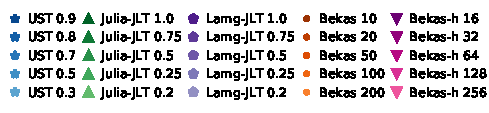
\includegraphics{sources/plots/el-clos/legend-quality.pdf}
\end{subfigure}\smallskip

\begin{subfigure}{.3\textwidth}
\centering
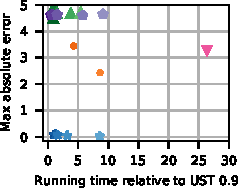
\includegraphics[width=\textwidth]{sources/plots/el-clos/abs-errors.pdf}
\caption{Maximum of the maximum absolute errors.}
\label{fig:el-clos:el-clos-max-abs}
\end{subfigure}\hfill
\begin{subfigure}{.3\textwidth}
\centering
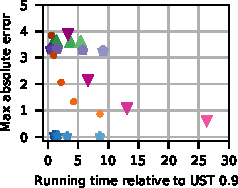
\includegraphics[width=\textwidth]{sources/plots/el-clos/avg-abs-errors.pdf}
\caption{Arithmetic mean of the maximum absolute error.}
\label{fig:el-clos:el-clos-avg-abs}
\end{subfigure}\hfill
\begin{subfigure}{.3\textwidth}
\centering
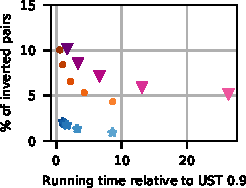
\includegraphics[width=\textwidth]{sources/plots/el-clos/full-ranking.pdf}
\caption{Geometric mean of the percentage of inverted pairs
in the full ranking of $\diag{\Linv}$.}
\label{fig:el-clos:el-clos-full-rank}
\end{subfigure}

\caption{Quality measures over the instances of \Cref{tab:el-clos:insts-ec-med-gt}.
All runs are sequential.}
\label{fig:el-clos:el-clos-quality}
\end{figure}

\Cref{fig:el-clos:el-clos-max-abs} shows that, in terms of maximum absolute error,
every configuration of \ust achieves results with higher quality than the competitors.
Even when setting $\epsilon = \numprint{0.9}$, \ust yields a maximum absolute
error of \ustMaxAbsErr, and it is \ustBekasSpeedup faster than \bekas with 200
random vectors -- which, in turn, achieves a maximum absolute error of \bekasMaxAbsErr.
Furthermore, the running time of \ust does not increase substantially for lower
values of $\epsilon$ and its quality does not deteriorate quickly for higher
values of $\epsilon$.
Regarding the average of the maximum absolute error,
\Cref{fig:el-clos:el-clos-avg-abs} shows that, among the competitors, \bekash
with 256 Hadamard rows achieves the best precision. \ust, however, yields an
average error of \ustAvgAbsErr while also being \ustBekasHSpeedup faster than
\bekash, which yields an average error of \bekasAvgAbsErr. Note also that the
number next to each method in \Cref{fig:el-clos:el-clos-quality} corresponds to
different values of absolute (for \ust) or relative (for \lamgjlt and
\juliajlt) error bounds, and different number of samples (for \bekas and
\bekash). For \bekash, the number of samples needs to be a multiple of four due
to dimension of Hadamard matrices.

In \Cref{fig:el-clos:el-clos-full-rank}, we report the percentage of inverted
pairs in the full ranking of the vertices according to $\diag{\Linvapx}$.
Note that JLT-based approaches are not depicted in this plot because they
yield $>15\%$ of rank inversions. Among the competitors, \bekas achieves the
best time-accuracy trade-off. However, when using 200 random vectors, it yields
\bekasRanking inversions while also being \ustBekasSpeedup slower than \ust
with $\epsilon = 0.9$, which yields \ustRanking inversions only.

For validation purposes, we also measure how well the considered algorithms
compute the \emph{set} (not the ranking) of top-$k$ vertices, \ie those with
highest electrical closeness centrality, with $k\in \set{10, 100}$. For each
algorithm we only consider the parameter settings that yields the highest
accuracy. JLT-based approaches appear to be very accurate for this purpose, as
their top-$k$ sets achieve a Jaccard index of $1.0$. As expected (due to its
absolute error guarantee), \ust performs slightly worse: on average, it obtains
\numprint{0.95} for $k = 10$ and \numprint{0.98} for $k = 100$, which still
shows a high overlap with the ground truth.

\subsection{Memory Consumption}
\begin{figure}[tb]
\centering
\begin{subfigure}{\textwidth}
\centering

\includegraphics{sources/plots/el-clos/legend-memory-consumption.pdf}
\end{subfigure}

\begin{subfigure}{.6\textwidth}
\centering
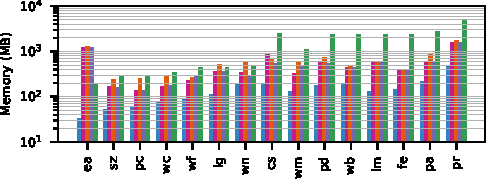
\includegraphics[width=\textwidth]{sources/plots/el-clos/memory-consumption.pdf}
\end{subfigure}
\caption{Difference between the peak resident set size before and after
a sequential run of each algorithm on the instances of
\Cref{tab:el-clos:insts-ec-med-gt,tab:el-clos:insts-ec-med-no-gt}.}
\label{fig:el-clos:memory}
\end{figure}

We measure the peak memory consumption of all the algorithms while running
sequentially on the instances of
\Cref{tab:el-clos:insts-ec-med-gt,tab:el-clos:insts-ec-med-no-gt}.
More precisely, we subtract the peak resident set size before launching
the algorithm from the peak resident size after the algorithm finished.
\Cref{fig:el-clos:memory} shows that \ust requires less memory than the
competitors on all the considered instances. This can be explained by the
fact that, unlike its competitors, our algorithm does not rely on Laplacian
solvers with considerable memory overhead.
For the largest network in particular, the peak memory is \ustMemPR MB for
\ust, and at least \lamgMemPR GB for the competitors.

\subsection{Parallel Scalability}
\label{sec:el-clos:par-scal}
\begin{figure}[tb]
\centering
\begin{subfigure}[t]{.45\textwidth}
\centering
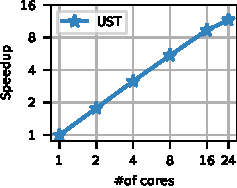
\includegraphics[width=.7\textwidth]{sources/plots/el-clos/ust-sh-mem-scalability.pdf}
\caption{Geometric mean of the speedup of \ust on multiple cores (shared memory)
\wrt a sequential run. Data points are aggregated over the instances of
\Cref{tab:el-clos:insts-ec-med-gt,tab:el-clos:insts-ec-med-no-gt}.}
\label{fig:el-clos:el-clos-sh-mem-scal}
\end{subfigure}\hfill
\begin{subfigure}[t]{.45\textwidth}
\centering
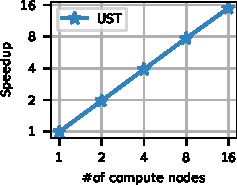
\includegraphics[width=.7\textwidth]{sources/plots/el-clos/ust-distr-mem-scalability.pdf}
\caption{Geometric mean of the speedup of \ust on multiple compute nodes
\wrt \ust on a single compute node ($1\times 24$ cores). Data points
are aggregated over the instances of \Crefrange{tab:el-clos:insts-ec-med-gt}{tab:el-clos:insts-ec-large}.}
\label{fig:el-clos:el-clos-distr-mem-scal}
\end{subfigure}
\caption{Parallel scalability of \ust (with $\epsilon = \numprint{0.3}$) with shared
and with distributed memory.}
\end{figure}

The log-log plot in \Cref{fig:el-clos:el-clos-sh-mem-scal} shows that, on shared memory,
\ust achieves a moderate parallel scalability \wrt the number of cores; on 24 cores in
particular, it is \shmemspeedup faster than on a single core.
Even though the number of USTs to be sampled can be evenly divided among the available
cores, we do not see a nearly-linear scalability: on multiple cores the memory performance
of our NUMA system becomes a bottleneck. Therefore, the time to sample a UST increases
and using more cores yields diminishing returns.
Limited memory bandwidth is a known issue affecting algorithms based on graph traversals
in general~\cite{DBLP:conf/icpp/BaderCF05,DBLP:journals/ppl/LumsdaineGHB07}.

Finally, we compare the parallel performance of \ust indirectly with the
parallel performance of our competitors. Specifically, assuming a perfect
parallel scalability for our competitors \bekas and \bekash on 24 cores, \ust
would yield results \numprint{4.1} and \numprint{12.6} times faster,
respectively, even with this strong assumption for the competition's benefit.

\ust scales better in a distributed setting. In this case, the scalability is affected
mainly by its non-parallel parts and by synchronization latencies.
The log-log plot in \Cref{fig:el-clos:el-clos-distr-mem-scal} shows that, on up to 4
compute nodes, the scalability is almost linear, while on 16 compute nodes \ust
achieves a \distrspeedup speedup \wrt a single compute node.

\begin{figure}[tb]
\centering
\begin{subfigure}[c]{.3\textwidth}
\centering
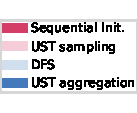
\includegraphics[width=.5\textwidth]{sources/plots/el-clos/legend-time-breakdown.pdf}
\end{subfigure}\hfill
\begin{subfigure}[c]{.6\textwidth}
\centering
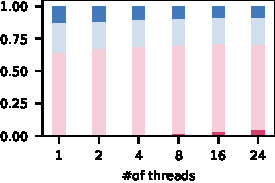
\includegraphics[width=.7\textwidth]{sources/plots/el-clos/time-breakdown.pdf}
\end{subfigure}
\caption{Breakdown of the running times of \ust with $\epsilon = \numprint{0.3}$
\wrt \#of cores on $1\times 24$ cores. Data is aggregated with the geometric
mean over the instances of \Cref{tab:el-clos:insts-ec-med-gt,tab:el-clos:insts-ec-med-no-gt}.}
\label{fig:el-clos:time-breakdown}
\end{figure}

\Cref{fig:el-clos:time-breakdown} shows the fraction of time \ust spends on
different tasks depending on the number of cores. We aggregated over
\enquote{Sequential Init.} the time spent on memory allocation, pivot
selection, solving the linear system, the computation of the biconnected
components, and on computing the BFS tree $B_u$. In all configurations, \ust
spends the majority of the time in sampling, computing the DFS data structures,
and aggregating USTs. The total time spent on aggregation corresponds to
\enquote{UST aggregation} and \enquote{DFS} in
\Cref{fig:el-clos:time-breakdown}, indicating that computing the DFS data
structures is the most expensive part of the aggregation. Together, sampling
time and aggregation time account for \ustFracOneCore and \ustFracAllCores of
the total running time on 1 core and 24 cores, respectively. On average,
sampling takes \avgSampling of this time, while total aggregation takes
\avgAggregate. Since sampling a UST is on average \aggOverSampl more expensive
than computing the DFS timestamps and aggregation, faster sampling techniques
would significantly improve the performance of our algorithm.

\subsection{Scalability to Large Networks}
\begin{figure}[tb]
\centering
\begin{subfigure}[t]{.45\textwidth}
\centering
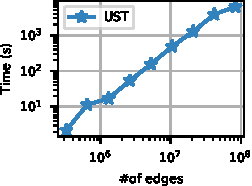
\includegraphics[width=.7\textwidth]{sources/plots/el-clos/hyp-scalability.pdf}
\caption{Running time of \ust \wrt \#of edges.}
\label{fig:el-clos:hyp-running-time}
\end{subfigure}\hfill
\begin{subfigure}[t]{.45\textwidth}
\centering
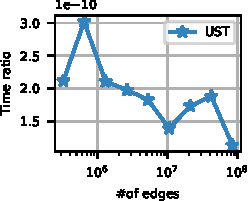
\includegraphics[width=.7\textwidth]{sources/plots/el-clos/hyp-theoretical-scalability.pdf}
\caption{Ratio between the running time of \ust and its theoretical running
time (see \Cref{theo:el-clos:diag-apx-algo}.}
\label{fig:el-clos:hyp-theo-running-time}
\end{subfigure}
\caption{Scalability of \ust on random hyperbolic graphs ($\epsilon = \numprint{0.3}$,
$1\times 24$ cores).}
\end{figure}

\begin{figure}[tb]
\centering
\begin{subfigure}[t]{.45\textwidth}
\centering
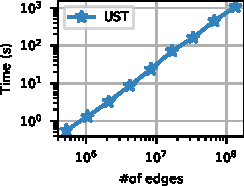
\includegraphics[width=.7\textwidth]{sources/plots/el-clos/rmat-scalability.pdf}
\caption{Running time of \ust \wrt \#of edges.}
\label{fig:el-clos:rmat-running-time}
\end{subfigure}\hfill
\begin{subfigure}[t]{.45\textwidth}
\centering
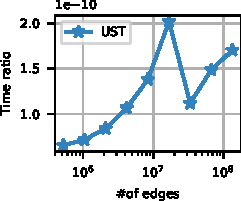
\includegraphics[width=.7\textwidth]{sources/plots/el-clos/rmat-theoretical-scalability.pdf}
\caption{Ratio between the running time of \ust and its theoretical running
time (see \Cref{theo:el-clos:diag-apx-algo}.}
\label{fig:el-clos:rmat-theo-running-time}
\end{subfigure}
\caption{Scalability of \ust on R-MAT graphs ($\epsilon = \numprint{0.3}$,
$1\times 24$ cores).}
\label{fig:el-clos:rmat-scalability}
\end{figure}

\paragraph{Results on Synthetic Networks}
The log-log plot in \Cref{fig:el-clos:hyp-running-time} show the average running time
of \ust $1\times24$ cores on random hyperbolic
networks~\cite{DBLP:conf/hpec/LoozOLM16}.\footnote{The random hyperbolic generator generates
networks with a heavy-tailed degree distribution. We set the average degree to 20 and the
exponent of the power-law distribution to 3.}
For each network size, we take the arithmetic mean of the running times
measured on five different randomly generated networks.
Our algorithm requires \maxTimeHyp minutes for the largest inputs
-- with up to \maxEdgesHyp million edges.
Interestingly, \Cref{fig:el-clos:hyp-theo-running-time} shows that the algorithm
scales slightly better than our theoretical bound predicts.
In \Cref{fig:el-clos:rmat-scalability} we present additional results on R-MAT
graphs~\cite{DBLP:conf/sdm/ChakrabartiZF04}. For this experiment, we use the
Graph 500~\cite{murphy2010introducing} parameter setting -- \ie \graphfh.
On these instances, the algorithm requires only \maxTimeRmat minutes on inputs
with up to \maxEdgesRmat million edges.
In particular, since these graphs have a nearly-constant diameter,
our algorithm is faster than on random hyperbolic graphs.
Qualitatively, it exhibits a similar scalability. The comparison to the theoretical
bound is, however, less conclusive.

\paragraph{Results on Large Real-World Networks}
\begin{table}[tb]
\centering
\small
\captionabove{Running time (s) of \ust on large real-world networks ($16\times 24$ cores).}
\label{tab:el-clos:el-clos-time-cluster}
\begin{tabular}{lrrrr}
\toprule
\multirow{2}{*}{Network} & \multirow{2}{*}{$n$} & \multirow{2}{*}{$m$} & Time (s)  & Time (s) \\
& & & $\epsilon = 0.3$ & $\epsilon = 0.9$ \\
\midrule
petster-carnivore & \numprint{601213} & \numprint{15661775} & \numprint{16.8} & \numprint{4.8}\\
soc-pokec-relationships & \numprint{1632803} & \numprint{22301964} & \numprint{55.5} & \numprint{9.5}\\
soc-LiveJournal1 & \numprint{4843953} & \numprint{42845684} & \numprint{277.0} & \numprint{75.5}\\
livejournal-links & \numprint{5189808} & \numprint{48687945} & \numprint{458.4} & \numprint{80.6}\\
orkut-links & \numprint{3072441} & \numprint{117184899} & \numprint{71.8} & \numprint{19.9}\\
wikipedia\_link\_en & \numprint{13591759} & \numprint{334590793} & \numprint{429.9} & \numprint{88.3}\\
\bottomrule
\end{tabular}
% Generated on: 20/04/2020 22:31:22

\end{table}

In \Cref{tab:el-clos:el-clos-time-cluster} we report the performance of \ust in
a distributed setting ($16\times 24$ cores) on large \emph{real-world} networks.
With $\epsilon = \numprint{0.3}$ and $\epsilon = \numprint{0.9}$, \ust always runs
in less than 8 minutes and $\numprint{1.5}$ minutes, respectively.

\subsection{Additional Experimental Results}
\label{sec:el-clos:rel-err-results}
\paragraph{Relative Error Quality Measures}
Because our algorithm computes an absolute $\pm\epsilon$-approximation of
$\diag{\Linv}$ with high probability, it is expected to yield better
results in terms of maximum absolute error and ranking than numerical approaches
with a relative error guarantee. Indeed, as we show in the following,
the quality assessment changes if we consider quality measures on a relative
error such as:

\begin{align*}
\lonerel &:= \frac{\onenorm{\diag{\Linv} - \diag{\Linvapx}}}{\onenorm{\diag{\Linv}}},\\
\ltworel &:= \frac{\twonorm{\diag{\Linv} - \diag{\Linvapx}}}{\twonorm{\diag{\Linv}}},\\
\erel &:= \text{gmean}_v\frac{\left|\Linv[v, v] - \Linvapx[v, v]\right|}{\Linv[v, v]}.
\end{align*}

\paragraph{Quality in terms of Relative Error}
\begin{figure}[tb]
\centering
\begin{subfigure}{\textwidth}
\centering
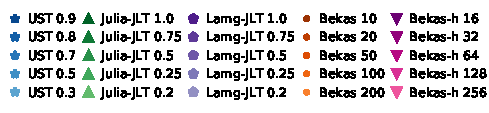
\includegraphics{sources/plots/el-clos/legend-quality.pdf}
\end{subfigure}\smallskip

\begin{subfigure}{.3\textwidth}
\centering
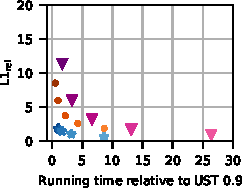
\includegraphics[width=\textwidth]{sources/plots/el-clos/l1-norm.pdf}
\end{subfigure}\hfill
\begin{subfigure}{.3\textwidth}
\centering
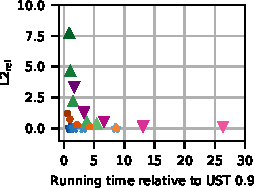
\includegraphics[width=\textwidth]{sources/plots/el-clos/l2-norm.pdf}
\end{subfigure}\hfill
\begin{subfigure}{.3\textwidth}
\centering
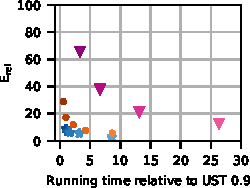
\includegraphics[width=\textwidth]{sources/plots/el-clos/relative-error.pdf}
\end{subfigure}
\caption{$\lonerel$, $\ltworel$, and $\erel$ \wrt the running time of our algorithm
with $\epsilon = \numprint{0.9}$. All data points are aggregated using the geometric
mean over the instances of \Cref{tab:el-clos:insts-ec-med-gt}.}
\label{fig:el-clos:el-clos-quality-rel}
\end{figure}

\Cref{fig:el-clos:el-clos-quality-rel} shows that, when assessing the error in
terms of $\lonerel$, $\ltworel$, or $\erel$, for the same running time, \ust
yields results that are still better in terms of quality than the competitors',
but not by such a wide margin. This can be explained by the fact that the numerical
solvers used by our competitors often employ measures analogous to $\lonerel$
and $\ltworel$ in their stopping conditions.

\section{Experiments -- Forest Closeness}
\label{sec:el-clos:exp-forest}

We now study the empirical performance of our algorithm for forest closeness
(\Cref{sec:el-clos:forest-clos-extension}) on real-world graphs.

\paragraph{Settings} Unless stated otherwise, all algorithms are implemented
in C++, using the NetworKit~\cite{DBLP:journals/netsci/StaudtSM16} graph APIs.
All experiments are conducted on Linux machines equipped with an \CPU
and \RAM each. Unless stated otherwise, all experiments run on a single core.
We manage our experiments with the SimexPal
software~\cite{DBLP:journals/algorithms/AngrimanGLMNPT19} to ensure
reproducibility. For evaluation, we use a large collection of undirected
graphs of different sizes, coming from a diverse set of domains. All graphs
have been downloaded from the public repositories KONECT~\cite{kunegis2013konect},
OpenStreetMap~\cite{OpenStreetMap}, and
NetworkRepository~\cite{DBLP:conf/aaai/RossiA15}.
We denote our proposed algorithm for forest closeness by \ust and,
as done in~\cite{DBLP:conf/icdm/JinBZ19}, we set $\alpha = 1$.

\paragraph{Competitors} For the forest closeness of individual
vertices, the main competitor is the JLT-based algorithm by
Jin \etal~\cite{DBLP:conf/icdm/JinBZ19}, which uses the Laplacian
solver from Ref.~\cite{DBLP:conf/focs/KyngS16}.
We compare against two implementations of this algorithm: one provided
by the authors written in Julia v1.0.2 and our own implementation
based on Eigen's~\cite{eigenweb} CG algorithm. We denote them by
\jltjulia and \jltcpp, respectively. Like in Ref.~\cite{DBLP:conf/icdm/JinBZ19},
we compute the number of linear systems for \jltjulia and \jltcpp
as $\ceil{\frac{\log n}{\epsilon^2}}$ -- which gives an
$(\epsilon\cdot c)$-approximation for a fixed constant $c > 1$.

\subsection{Performance of \ust}
We measure the performance of \ust compared to the state of the art.
Each method is executed with multiple settings of its respective quality
parameter.

\paragraph{Accuracy and Running Time}
\begin{table}[tb]
\setlength{\tabcolsep}{2pt}
\centering
\footnotesize
\caption{Running time and KT ranking scores of \ust
and JLT-based algorithms. In the JLT column we report,
for each instance, the competitor with highest KT score.
For equal KT scores -- up to the second decimal place --
we choose the fastest competitor.}
\label{tab:el-clos:forest-corr}
\begin{subtable}[t]{.5\textwidth}
\centering
\caption{Complex networks}
\label{tab:el-clos:forest-corr-cplx}
\begin{tabular}{lrrrrrrr}
\toprule
\multirow{2}{*}{Graph} & \multirow{2}{*}{$n$} & \multirow{2}{*}{$m$} & \multicolumn{2}{c}{Time (s)} & \multicolumn{2}{c}{KT}\\
& & & UST & JLT & UST & JLT\\
\midrule
loc-brightkite\_edges & 58K & 214K& \textbf{\numprint{46.4}}& \numprint{186.4}& \textbf{\numprint{0.98}}& \numprint{0.95}\\
douban & 154K & 327K& \textbf{\numprint{80.8}}& \numprint{370.9}& \textbf{\numprint{0.71}}& \numprint{0.61}\\
soc-Epinions1 & 75K & 405K& \textbf{\numprint{55.5}}& \numprint{339.6}& \textbf{\numprint{0.95}}& \numprint{0.90}\\
slashdot-zoo & 79K & 467K& \textbf{\numprint{59.9}}& \numprint{412.3}& \textbf{\numprint{0.95}}& \numprint{0.92}\\
petster-cat-household & 105K & 494K& \textbf{\numprint{61.8}}& \numprint{372.1}& \textbf{\numprint{0.98}}& \numprint{0.92}\\
wikipedia\_link\_fy & 65K & 921K& \textbf{\numprint{58.2}}& \numprint{602.9}& \textbf{\numprint{0.98}}& \numprint{0.96}\\
loc-gowalla\_edges & 196K & 950K& \textbf{\numprint{230.9}}& \numprint{1215.5}& \textbf{\numprint{0.99}}& \numprint{0.97}\\
wikipedia\_link\_an & 56K & 1.1M& \textbf{\numprint{50.7}}& \numprint{562.6}& \textbf{\numprint{0.96}}& \numprint{0.93}\\
wikipedia\_link\_ga & 55K & 1.2M& \textbf{\numprint{44.8}}& \numprint{578.6}& \textbf{\numprint{0.98}}& \numprint{0.97}\\
petster-dog-household & 260K & 2.1M& \textbf{\numprint{359.6}}& \numprint{2472.1}& \textbf{\numprint{0.98}}& \numprint{0.96}\\
livemocha & 104K & 2.2M& \textbf{\numprint{107.4}}& \numprint{1429.3}& \textbf{\numprint{0.98}}& \numprint{0.97}\\
\bottomrule
\end{tabular}

\end{subtable}\hfill
\begin{subtable}[t]{.5\textwidth}
\centering
\caption{Road networks}
\label{tab:el-clos:forest-corr-road}
\begin{tabular}{lrrrrrrr}
\toprule
\multirow{2}{*}{Graph} & \multirow{2}{*}{$n$} & \multirow{2}{*}{$m$} & \multicolumn{2}{c}{Time (s)} & \multicolumn{2}{c}{KT}\\
& & & UST & JLT & UST & JLT\\
\midrule
mauritania & 102K & 150K& \textbf{\numprint{98.1}}& \numprint{217.6}& \textbf{\numprint{0.88}}& \numprint{0.77}\\
turkmenistan & 125K & 165K& \textbf{\numprint{118.5}}& \numprint{273.6}& \textbf{\numprint{0.92}}& \numprint{0.85}\\
cyprus & 151K & 189K& \textbf{\numprint{149.4}}& \numprint{315.8}& \textbf{\numprint{0.89}}& \numprint{0.80}\\
canary-islands & 169K & 208K& \textbf{\numprint{185.5}}& \numprint{382.0}& \textbf{\numprint{0.92}}& \numprint{0.84}\\
albania & 196K & 223K& \textbf{\numprint{192.6}}& \numprint{430.2}& \textbf{\numprint{0.90}}& \numprint{0.82}\\
benin & 177K & 234K& \textbf{\numprint{188.1}}& \numprint{406.8}& \textbf{\numprint{0.92}}& \numprint{0.83}\\
georgia & 262K & 319K& \textbf{\numprint{322.1}}& \numprint{605.3}& \textbf{\numprint{0.91}}& \numprint{0.83}\\
latvia & 275K & 323K& \textbf{\numprint{355.2}}& \numprint{665.4}& \textbf{\numprint{0.91}}& \numprint{0.83}\\
somalia & 291K & 409K& \textbf{\numprint{420.1}}& \numprint{747.5}& \textbf{\numprint{0.92}}& \numprint{0.84}\\
ethiopia & 443K & 607K& \textbf{\numprint{825.9}}& \numprint{1209.7}& \textbf{\numprint{0.91}}& \numprint{0.83}\\
tunisia & 568K & 766K& \textbf{\numprint{1200.1}}& \numprint{1629.0}& \textbf{\numprint{0.89}}& \numprint{0.79}\\
\bottomrule
\end{tabular}

\end{subtable}
\end{table}

We report the maximum absolute error of the estimated diagonal values
(\ie $\max_v|\Fmat[v, v] - \Fmatapx[v, v]|$) over all vertices and instances
from \Cref{tab:el-clos:forest-corr}.\footnote{Note that, as for electrical
closeness, the top vertices in the forest closeness ranking are the ones
with the \emph{lowest} $\Fmat[v,v]$ (see \Cref{eq:el-clos:forest-farness});
hence, we also evaluate the ranking accuracy in a following experiment.}
%
As ground truth, we take $\Fmat[v, v]$ values that are computed using
Eigen's~\cite{eigenweb} CG solver with a tolerance of $10^{-9}$;
exact inversion of $(\Lapl + \Ident)$ would be infeasible for many
of the input graphs. A preliminary comparison against the values
if $\Fmat[v, v]$ computed with the NumPy \texttt{pinv} function
demonstrated the CG provides a sufficiently accurate ground truth.

\begin{figure}[tb]
\centering
\begin{subfigure}[t]{\textwidth}
\centering
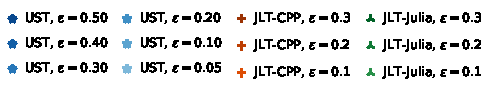
\includegraphics{sources/plots/el-clos/forest-quality-legend.pdf}
\end{subfigure}\smallskip

\begin{subfigure}[t]{.45\textwidth}
\centering
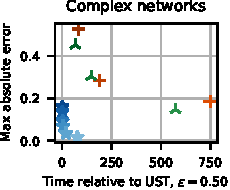
\includegraphics[width=.7\textwidth]{sources/plots/el-clos/forest-max-abs-err-cplx.pdf}
\end{subfigure}\hfill
\begin{subfigure}[t]{.45\textwidth}
\centering
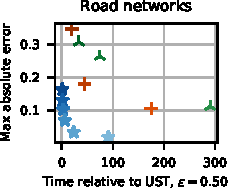
\includegraphics[width=.7\textwidth]{sources/plots/el-clos/forest-max-abs-err-road.pdf}
\end{subfigure}
\caption{$\max_v\left|\Fmat[v, v] - \Fmatapx[v, v]\right|$ over the instances
of \Cref{tab:el-clos:forest-corr}.}
\label{fig:el-clos:forest-quality}
\end{figure}

\Cref{fig:el-clos:forest-quality} shows that \ust achieves the best
results in terms of quality and running time for both complex and road
networks. More precisely, for complex networks and $\epsilon = 0.4$, \ust
yields a maximum absolute error of $\ustMaxAbsFour$, which is less than the
most accurate result of both competitors ($\jltJuliaMaxAbsOne$ achieved by
\jltjulia with $\epsilon = 0.1$), while being $\ustJuliaFourOneSpeedup$ faster.
Also, the running time of \ust does not increase substantially for
lower values of $\epsilon$, and its quality does not deteriorate quickly for
higher values of $\epsilon$. A similar pattern is observed for road networks as
well. Detailed running time values are reported in \Cref{tab:el-clos:forest-time},
\Cref{apx:el-clos:forest-time}.

\paragraph{Vertex Ranking} Moreover, we measure the accuracy in terms of
vertex rankings, which is often more relevant than individual
scores~\cite{DBLP:conf/faw/OkamotoCL08,newman2018networks}.
In \Cref{tab:el-clos:forest-corr}, we report the Kendall's rank correlation
coefficient (KT) of the vertex ranking \wrt the ground truth along with
running times for complex networks (\Cref{tab:el-clos:forest-corr-cplx})
and for road networks (\Cref{tab:el-clos:forest-corr-road}).
%
For each instance, we pick the best run, \ie the \enquote{UST} and
\enquote{JLT} columns display the run with highest respective KT value.
If the values are the same up to the second decimal place, we pick the
fastest one. \ust has consistently the best vertex ranking scores;
at the same time, it is faster than the competitors. In particular,
\ust is on average $\ustJLTSpeedupCplx$ faster than the JLT-based approaches
on complex networks and $\ustJLTSpeedupRoad$ faster on road networks.

\paragraph{Parallel Scalability}
\begin{figure}[tb]
\centering
\begin{subfigure}[t]{.45\textwidth}
\centering
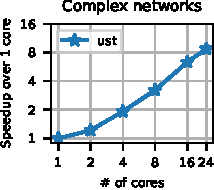
\includegraphics[width=.7\textwidth]{sources/plots/el-clos/parallel-scalability-forest-cplx.pdf}
\end{subfigure}\hfill
\begin{subfigure}[t]{.45\textwidth}
\centering
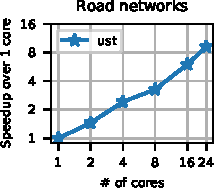
\includegraphics[width=.7\textwidth]{sources/plots/el-clos/parallel-scalability-forest-road.pdf}
\end{subfigure}
\caption{Geometric mean of the speedup of \ust with $\epsilon = \numprint{0.05}$
on multiple cores over a sequential run (shared memory).
Data points are aggregated over the instances of \Cref{tab:el-clos:forest-corr}.}
\label{fig:el-clos:forest-par-scal}
\end{figure}

\begin{figure}[tb]
\centering
\begin{subfigure}[t]{.45\textwidth}
\centering
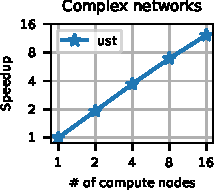
\includegraphics[width=.7\textwidth]{sources/plots/el-clos/distributed-scalability-forest-cplx.pdf}
\end{subfigure}\hfill
\begin{subfigure}[t]{.45\textwidth}
\centering
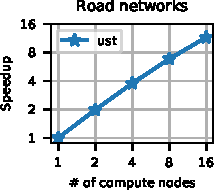
\includegraphics[width=.7\textwidth]{sources/plots/el-clos/distributed-scalability-forest-road.pdf}
\end{subfigure}
\caption{Geometric mean of the speedup of \ust with $\epsilon = \numprint{0.1}$
on multiple compute nodes over a single compute node ($1\times 24$ cores).
Data points are aggregated over the instances of \Cref{tab:el-clos:insts-forest-large}.}
\label{fig:el-clos:forest-distr-scal}
\end{figure}

\begin{table}[tb]
\centering\footnotesize
\setlength{\tabcolsep}{2pt}
\captionabove{Large networks used for scalability experiments
in distributed memory and running time of \ust for forest closeness
on $16\times 24$ cores.}
\label{tab:el-clos:insts-forest-large}
\begin{subtable}[t]{.5\textwidth}
\centering
\caption{Complex networks}
\begin{tabular}{lrrrr}
\toprule
\multirow{2}{*}{Graph} & \multirow{2}{*}{$n$} & \multirow{2}{*}{$m$} & \multicolumn{2}{c}{Time (s)} \\
                       & & & $\epsilon = \numprint{0.1}$ & $\epsilon = \numprint{0.3}$\\
\midrule
soc-LiveJournal1 & \numprint{4846609} & \numprint{42851237} & \numprint{348.9} & \numprint{118.5}\\
wikipedia\_link\_fr & \numprint{3333397} & \numprint{100461905} & \numprint{205.4} & \numprint{90.7}\\
orkut-links & \numprint{3072441} & \numprint{117184899} & \numprint{293.5} & \numprint{92.2}\\
dimacs10-uk-2002 & \numprint{18483186} & \numprint{261787258} & \numprint{1101.3} & \numprint{365.8}\\
wikipedia\_link\_en & \numprint{13593032} & \numprint{334591525} & \numprint{919.3} & \numprint{295.4}\\
\bottomrule
\end{tabular}

\end{subtable}\hfill
\begin{subtable}[t]{.5\textwidth}
\centering
\caption{Complex networks}
\begin{tabular}{lrrrr}
\toprule
\multirow{2}{*}{Graph} & \multirow{2}{*}{$n$} & \multirow{2}{*}{$m$} & \multicolumn{2}{c}{Time (s)} \\
 & & & $\varepsilon = 0.1$ & $\varepsilon = 0.3$\\
\midrule
slovakia & \numprint{543733} & \numprint{638114} & \numprint{28.1} & \numprint{9.9}\\
netherlands & \numprint{1437177} & \numprint{1737377} & \numprint{82.9} & \numprint{31.1}\\
greece & \numprint{1466727} & \numprint{1873857} & \numprint{74.5} & \numprint{29.8}\\
spain & \numprint{4557386} & \numprint{5905365} & \numprint{273.0} & \numprint{86.2}\\
great-britain & \numprint{7108301} & \numprint{8358289} & \numprint{419.0} & \numprint{136.6}\\
dach & \numprint{20207259} & \numprint{25398909} & \numprint{1430.1} & \numprint{473.7}\\
africa & \numprint{23975266} & \numprint{31044959} & \numprint{1493.4} & \numprint{499.3}\\
\bottomrule
\end{tabular}

\end{subtable}
\end{table}

As described in \Cref{sec:el-clos:par-impl}, \ust is well-suited for parallel
implementations since each UST can be sampled independently in parallel.
Hence, we provide parallel implementations of \ust based on OpenMP (for
multi-core parallelism) and MPI (to scale to multiple compute nodes)
for forest closeness as well.

In \Cref{fig:el-clos:forest-par-scal}, we report the parallel scalability of
\ust on multiple cores. Unsurprisingly, analogously to the results achieved in
\Cref{sec:el-clos:par-scal}, \ust exhibits a moderate scalability \wrt the
number of cores. In particular, our OpenMP implementation on 24 cores exhibits
a speedup of $\parSpeedupCplx$ on complex networks and $\parSpeedupRoad$ on
road networks. As with electrical closeness, we hypothesize that this is mainly
due to memory latencies: while sampling a UST, our algorithm performs several
random accesses to the graph data structure (\ie an adjacency
array~\cite{DBLP:journals/netsci/StaudtSM16}), which are prone to cache misses.
%
The results for MPI are depicted in \Cref{fig:el-clos:forest-distr-scal}.
In this setting, \ust obtains a speedup of
$\distrSpeedupCplx$ on complex and $\distrSpeedupRoad$ on road networks
on up to 16 compute nodes -- for this experiment we set $\epsilon = \numprint{0.1}$
and we use the instances in \Cref{tab:el-clos:insts-forest-large}.
More sophisticated load balancing techniques are likely to increase the speedup
in the MPI setting, they are left for future work.
Still, the MPI-based algorithm can rank complex networks with up to $334$M
edges in less than $20$ minutes. Road networks with $31$M edges take less than
$25$ minutes.

\section{Conclusions}
%
This chapter addressed the problem of approximating
electrical centrality measures, namely, electrical closeness, normalized
random-walk betweenness, Kirchhoff-related indices, and forest closeness. The
core contribution is a new efficient parallel algorithm for approximating
$\diag{\Linv}$ of Laplacian matrices \Lapl corresponding to small-world
weighted undirected networks, which is enough to compute the aforementioned
measures. Compared to the main competitors, our algorithm is about one order of
magnitude faster, it yields results with superior quality in terms of absolute
error and ranking of $\diag{\Linv}$, and it requires less memory.

Furthermore, we extended our algorithm to forest closeness, which can now be
approximated faster and more accurately than previously possible. Because the
augmented graph has constant diameter, in the forest closeness case we can
target any graph -- not only small-world graphs \change{-- without
degrading the performance of the algorithm}.

The gap between the theoretical bounds and the much better empirical error
yielded by our algorithm in approximating $\diag{\Linv}$ suggests that tighter
bounds on the number of samples are a promising direction for future research.
Another potentially interesting research direction is to devise a new
UST-based adaptive sampling strategy, as it could reduce the number of samples
and thus the running time of our \ust algorithm and it would benefit
from our epoch-based framework for parallel ADS described in
\Cref{ch:betweenness-approx}.
Other conceivable ideas for future work are an improvement of the running time
for high-diameter graphs, both in theory and in practice, and extensions of our
strategies to directed graphs.
